\documentclass[12pt]{article}
%--------------------   start of the 'preamble'
%
\usepackage{graphicx,amssymb,amstext,amsmath,color}
\usepackage[margin=2cm]{geometry}
\usepackage{abstract}
\usepackage{setspace}
\usepackage[footnotesize,bf]{caption}

% TABLE
\usepackage{multicol,hhline,colortbl,multirow}
\usepackage{braket}
\usepackage{siunitx}
\usepackage{hyperref}
\usepackage{authblk}
\usepackage{siunitx}
\usepackage{adjustbox}
\usepackage{mathrsfs}
%%\usepackage[sort&compress]{natbib}
%%\bibpunct{(}{)}{,}{a}{, }{;}
%
\usepackage[sort&compress]{natbib}
\bibpunct{[}{]}{,}{s}{}{;}


\definecolor{gray}{gray}{0.8}
\def\mobunits{\square\centi\meter\per\volt\per\second}
\def\gcm{\gram\per\cubic\centi\meter}
\def\ccg{\cellcolor{gray}}

\renewcommand{\labelitemii}{$\circ$}
\renewcommand{\bibname}{References}


\title{MorphCT Results - Voronoi Neighbour Analysis}
\author{Matthew Jones}
\date{\today}

\begin{document}
\maketitle

\section{Summary}

The following jobs have all been run using the new Voronoi cell neighbourlist calculation, rather than the radial cut-off that we used previously.

In order to test the full pipeline after the recent changes to MorphCT, I have both rerun the old morphologies using the new Voronoi cell neighbourlist calculation (origFG), as well as the complete pipeline again including a new fine-graining iteration (newFG).
The only differences between the origFG and newFG runs are the DPD parameters of the second molecular dynamics phase, which were softened in newFG to provide better results for PAHs and BDT-TPD.
Otherwise, the forcefields are identical.


\begin{itemize}
    \item{The mobility trends seem unaffected between cut-off and Voronoi.
            We still get the same 2-3 order of magnitude decrease in mobility from the ordered to disordered morphologies, as well as a general increase by 2 OOM on the mobility as the morphology evolves, which is in agreement with what we saw from the cut-off data.
            However, the absolute values of the mobility are quite different, with an increase of about 2 orders of magnitude across the board from the previous data.
            This is somewhat unusual, as we can safely expect that longer-range hops to next-nearest-neighbours are permitted in the cut-off case, but not when the neighbourlist is calculated through Voronoi analysis (which should only consider first-nearest-neighbour hops with adjacent Voronoi cells).
            Perhaps we were diluting our neighbour landscape by including slow, long-range hops, which were sometimes selected during the KMC, leading to a decreased overall mobility.
        }
    \item{The differences between the origFG and the newFG data looks pretty significant initially, but on closer inspection, the $T = 2.25$ data has a pretty horrible MSD fit.
            When this datapoint is treated as an outlier, the other disordered mobilities have similar values, each of which is about 1 order of magnitude lower than the ordered mobility.
            This difference is less than we observed previously using the cut-off, but still qualitatively suggests a dichotomy between the ordered and disordered simulations.
        Right now, I don't have much intuition why the $T = 2.25$ fit is so rough.
    I'm continuing to run the job for another 24 hours and see if it sorts itself out, but we'll have to see.}
    \item{The issue with the origFG temperature jobs has been rectified.
        The 3D connection heatmap \textbf{16} now looks like \textbf{30} as expected.}
\item{The anisotropies of \textbf{21-26} show that carriers aren't leaving the simulation volume.
    This is born out by the 3D heatmaps which show poorly connected domains and islands, and crappy MSD fits.
    This is somewhat unsurprising, given that the very disordered initial morphologies results in more islands and trapped charges.
}
\item{The Voronoi analysis has dramatically diminished all correlations between the order and the percentage of intra-chain hops performed, equalising the intra-chain proportion to 12\%-18\% across the board.
        Interestingly, this appears to have gone some way to solving our KMC sampling issue, where if the majority of high-hopping-rate hops are along the chain the trapping gets significantly worse.
        For instance, systems \textbf{2-5} have solely intra-molecular hops on the right hand side of the distribution, but still good anisotropies and MSD fits, whereas \textbf{6-15} have more balanced intra-/inter- hops at the high end but good anisotropies and MSD fits.
        It looks like cutting out the `next-nearest-intra-chain-neighbours' and beyond, which were available in the previous cut-off runs, has reduced the number of intra-chain hops overall and allowed us to continue to sample the inter-chain hops.
    }
\item{We must remember that ORCA only considers pairs of chromophores.
        Consider for example a line of 3 chromophores labelled A, B, and C, close enough that A and B have non-zero transfer integrals, as do B and C.
        We would expect transport to be good between A $\rightarrow$ B, B $\rightarrow$ C, but worse for A $\rightarrow$ C as there is a chromophore in the middle of them.
        If the separation between A and C is less than the cut-off, then A $\rightarrow$ C will be included and the transfer integral calculated.
        This would not be an issue, providing that $T_{AC} < T_{AB}$, however there is no guarantee of that because ORCA will only see the chromophores A and C, with no B in between them.
        We already know that orientation has a larger effect on the transfer integral than separation, so this could lead to $T_{AC} > T_{AB}$, making it a more preferential hop, and artificially increasing our mobility.
        Even if $T_{AC} \sim T_{AB}$, we must remember that the carrier is hopping further as $r_{AC} > r_{AB}$, which again can lead to an inflated mobility.
        The above also describes the issue with including every pair of chromophores in the system and letting ORCA decide whether the hops are important or not - because ORCA does not see any chromophores in between, its results cannot be trusted beyond nearest-neighbour hops.
        Voronoi analysis guarantees that we only consider these nearest-neighbour hops and removes this problem entirely, which is why I believe our results are more physical using it, even if they approximate the experimental results less accurately.
    }
\end{itemize}




\begin{center}
\begin{adjustbox}{max width=\textwidth}
\begin{tabular}{| c | c | c | c | c | c | c |}
\hline
\rule{0pt}{2.5ex} 
\multirow{2}{*}{\textbf{ID}}&\multirow{2}{*}{\textbf{Simulation Name}}&\textbf{Density}&\textbf{Anisotropy}&\textbf{Anisotropy}&\textbf{Mobility}&\textbf{Intra-}\\
                            &&(\SI{}{\gcm})&(Arb. U.)&(Shape)&(\SI{}{\mobunits})&\textbf{\%}\\
\hhline{|=======|}
\multicolumn{7}{| c |}{{\ccg}NewFG Runs}\\
\hhline{|=======|}
\textbf{1}&\rule{0pt}{2.5ex}newFG-p1-L15-f0.0-P0.1-T1.5-e0.5&1.676&0.0676&---&1.17$\times 10^{1}$&12.53\%\\
{\ccg}\textbf{2}&{\ccg}\rule{0pt}{2.5ex}newFG-p1-L15-f0.0-P0.1-T1.75-e0.5&{\ccg}1.061&{\ccg}0.0065&{\ccg}Spherical&{\ccg}3.48$\times 10^{-1}$&{\ccg}17.59\%\\
\textbf{3}&\rule{0pt}{2.5ex}newFG-p1-L15-f0.0-P0.1-T2.0-e0.5&0.892&0.0026&Spherical&4.46$\times 10^{-1}$&17.58\%\\
{\ccg}\textbf{4}&{\ccg}\rule{0pt}{2.5ex}newFG-p1-L15-f0.0-P0.1-T2.25-e0.5&{\ccg}0.787&{\ccg}0.0044&{\ccg}Spherical&{\ccg}5.52$\times 10^{-1}$&{\ccg}17.83\%\\
\textbf{5}&\rule{0pt}{2.5ex}newFG-p1-L15-f0.0-P0.1-T2.5-e0.5&0.685&0.0041&Spherical&4.03$\times 10^{-1}$&18.00\%\\
\hhline{|=======|}
{\ccg}\textbf{6}&{\ccg}\rule{0pt}{2.5ex}newFG-0001\_withImages&{\ccg}1.061&{\ccg}0.0059&{\ccg}Spherical&{\ccg}2.65$\times 10^{-1}$&{\ccg}17.46\%\\
\textbf{7}&\rule{0pt}{2.5ex}newFG-0005\_withImages&1.336&0.0077&Spherical&4.68$\times 10^{-2}$&13.34\%\\
{\ccg}\textbf{8}&{\ccg}\rule{0pt}{2.5ex}newFG-0010\_withImages&{\ccg}1.345&{\ccg}0.0063&{\ccg}Spherical&{\ccg}7.50$\times 10^{-1}$&{\ccg}13.73\%\\
\textbf{9}&\rule{0pt}{2.5ex}newFG-0020\_withImages&1.428&0.0137&Spherical&1.22$\times 10^{0}$&13.23\%\\
{\ccg}\textbf{10}&{\ccg}\rule{0pt}{2.5ex}newFG-0040\_withImages&{\ccg}1.450&{\ccg}0.0077&{\ccg}Spherical&{\ccg}7.92$\times 10^{-2}$&{\ccg}13.78\%\\
\textbf{11}&\rule{0pt}{2.5ex}newFG-0100\_withImages&1.510&0.0228&Spherical&4.33$\times 10^{0}$&12.89\%\\
{\ccg}\textbf{12}&{\ccg}\rule{0pt}{2.5ex}newFG-0200\_withImages&{\ccg}1.554&{\ccg}0.0721&{\ccg}Ellipsoid&{\ccg}4.94$\times 10^{0}$&{\ccg}12.74\%\\
\textbf{13}&\rule{0pt}{2.5ex}newFG-0300\_withImages&1.593&0.1041&Disk&6.44$\times 10^{0}$&12.61\%\\
{\ccg}\textbf{14}&{\ccg}\rule{0pt}{2.5ex}newFG-0500\_withImages&{\ccg}1.638&{\ccg}0.1186&{\ccg}Disk&{\ccg}9.26$\times 10^{0}$&{\ccg}12.55\%\\
\textbf{15}&\rule{0pt}{2.5ex}newFG-1000\_withImages&1.662&0.0957&Disk&9.11$\times 10^{0}$&12.49\%\\
\hhline{|=======|}
\multicolumn{7}{| c |}{{\ccg}OrigFG Runs}\\
\hhline{|=======|}
\textbf{16}&\rule{0pt}{2.5ex}origFG-p1-L15-f0.0-P0.1-T1.5-e0.5&1.676&0.1074&Disk&$8.06\times 10^{0}$&12.67\%\\
{\ccg}\textbf{17}&{\ccg}\rule{0pt}{2.5ex}origFG-p1-L15-f0.0-P0.1-T1.75-e0.5&{\ccg}1.061&{\ccg}0.0038&{\ccg}Spherical&{\ccg}5.18$\times 10^{-1}$&{\ccg}17.38\%\\
\textbf{18}&\rule{0pt}{2.5ex}origFG-p1-L15-f0.0-P0.1-T2.0-e0.5&0.892&0.0023&Spherical&4.36$\times 10^{-1}$&17.72\%\\
{\ccg}\textbf{19}&{\ccg}\rule{0pt}{2.5ex}origFG-p1-L15-f0.0-P0.1-T2.25-e0.5&{\ccg}0.787&{\ccg}0.0038&{\ccg}Spherical&{\ccg}3.20$\times 10^{-2}$&{\ccg}18.12\%\\
\textbf{20}&\rule{0pt}{2.5ex}origFG-p1-L15-f0.0-P0.1-T2.5-e0.5&0.685&0.0031&Spherical&4.00$\times 10^{-1}$&18.44\%\\
\hhline{|=======|}
{\ccg}\textbf{21}&{\ccg}\rule{0pt}{2.5ex}origFG-0001\_withImages&{\ccg} 1.061&{\ccg}0.0045&{\ccg}Spherical&{\ccg}$1.73\times 10^{-1}$&{\ccg}17.50\%\\
\textbf{22}&\rule{0pt}{2.5ex}origFG-0005\_withImages&1.336&0.0041&Spherical&1.00$\times 10^{-2}$&16.97\%\\
{\ccg}\textbf{23}&{\ccg}\rule{0pt}{2.5ex}origFG-0010\_withImages&{\ccg} 1.345&{\ccg}0.0073&{\ccg}Spherical&{\ccg}4.06$\times 10^{-2}$&{\ccg}16.99\%\\
\textbf{24}&\rule{0pt}{2.5ex}origFG-0020\_withImages&1.428&0.0107&Spherical&1.84$\times 10^{-2}$&17.13\%\\
{\ccg}\textbf{25}&{\ccg}\rule{0pt}{2.5ex}origFG-0040\_withImages&{\ccg} 1.450&{\ccg}0.0112&{\ccg}Spherical&{\ccg}1.68$\times 10^{-2}$&{\ccg}16.89\%\\
\textbf{26}&\rule{0pt}{2.5ex}origFG-0100\_withImages&1.510&0.0154&Spherical&2.79$\times 10^{-2}$&14.28\%\\
{\ccg}\textbf{27}&{\ccg}\rule{0pt}{2.5ex}origFG-0200\_withImages&{\ccg} 1.554&{\ccg}0.0631&{\ccg}Ellipsoid&{\ccg}$1.72\times 10^{0}$&{\ccg}13.19\%\\
\textbf{28}&\rule{0pt}{2.5ex}origFG-0300\_withImages&1.593&0.1113&Disk&1.09$\times 10^{0}$&12.99\%\\
{\ccg}\textbf{29}&{\ccg}\rule{0pt}{2.5ex}origFG-0500\_withImages&{\ccg} 1.638&{\ccg}0.1013&{\ccg}Disk&{\ccg}4.73$\times 10^{0}$&{\ccg}12.69\%\\
\textbf{30}&\rule{0pt}{2.5ex}origFG-1000\_withImages&1.662&0.1025&Disk&2.74$\times 10^{0}$&12.64\%\\
\hhline{-------}
\end{tabular}\label{table:mob}
\end{adjustbox}
\captionof{table}{The latest results obtained when using the new Voronoi cell neighbourlist calculation.}
\end{center}

\begin{figure}[h!]\centering
	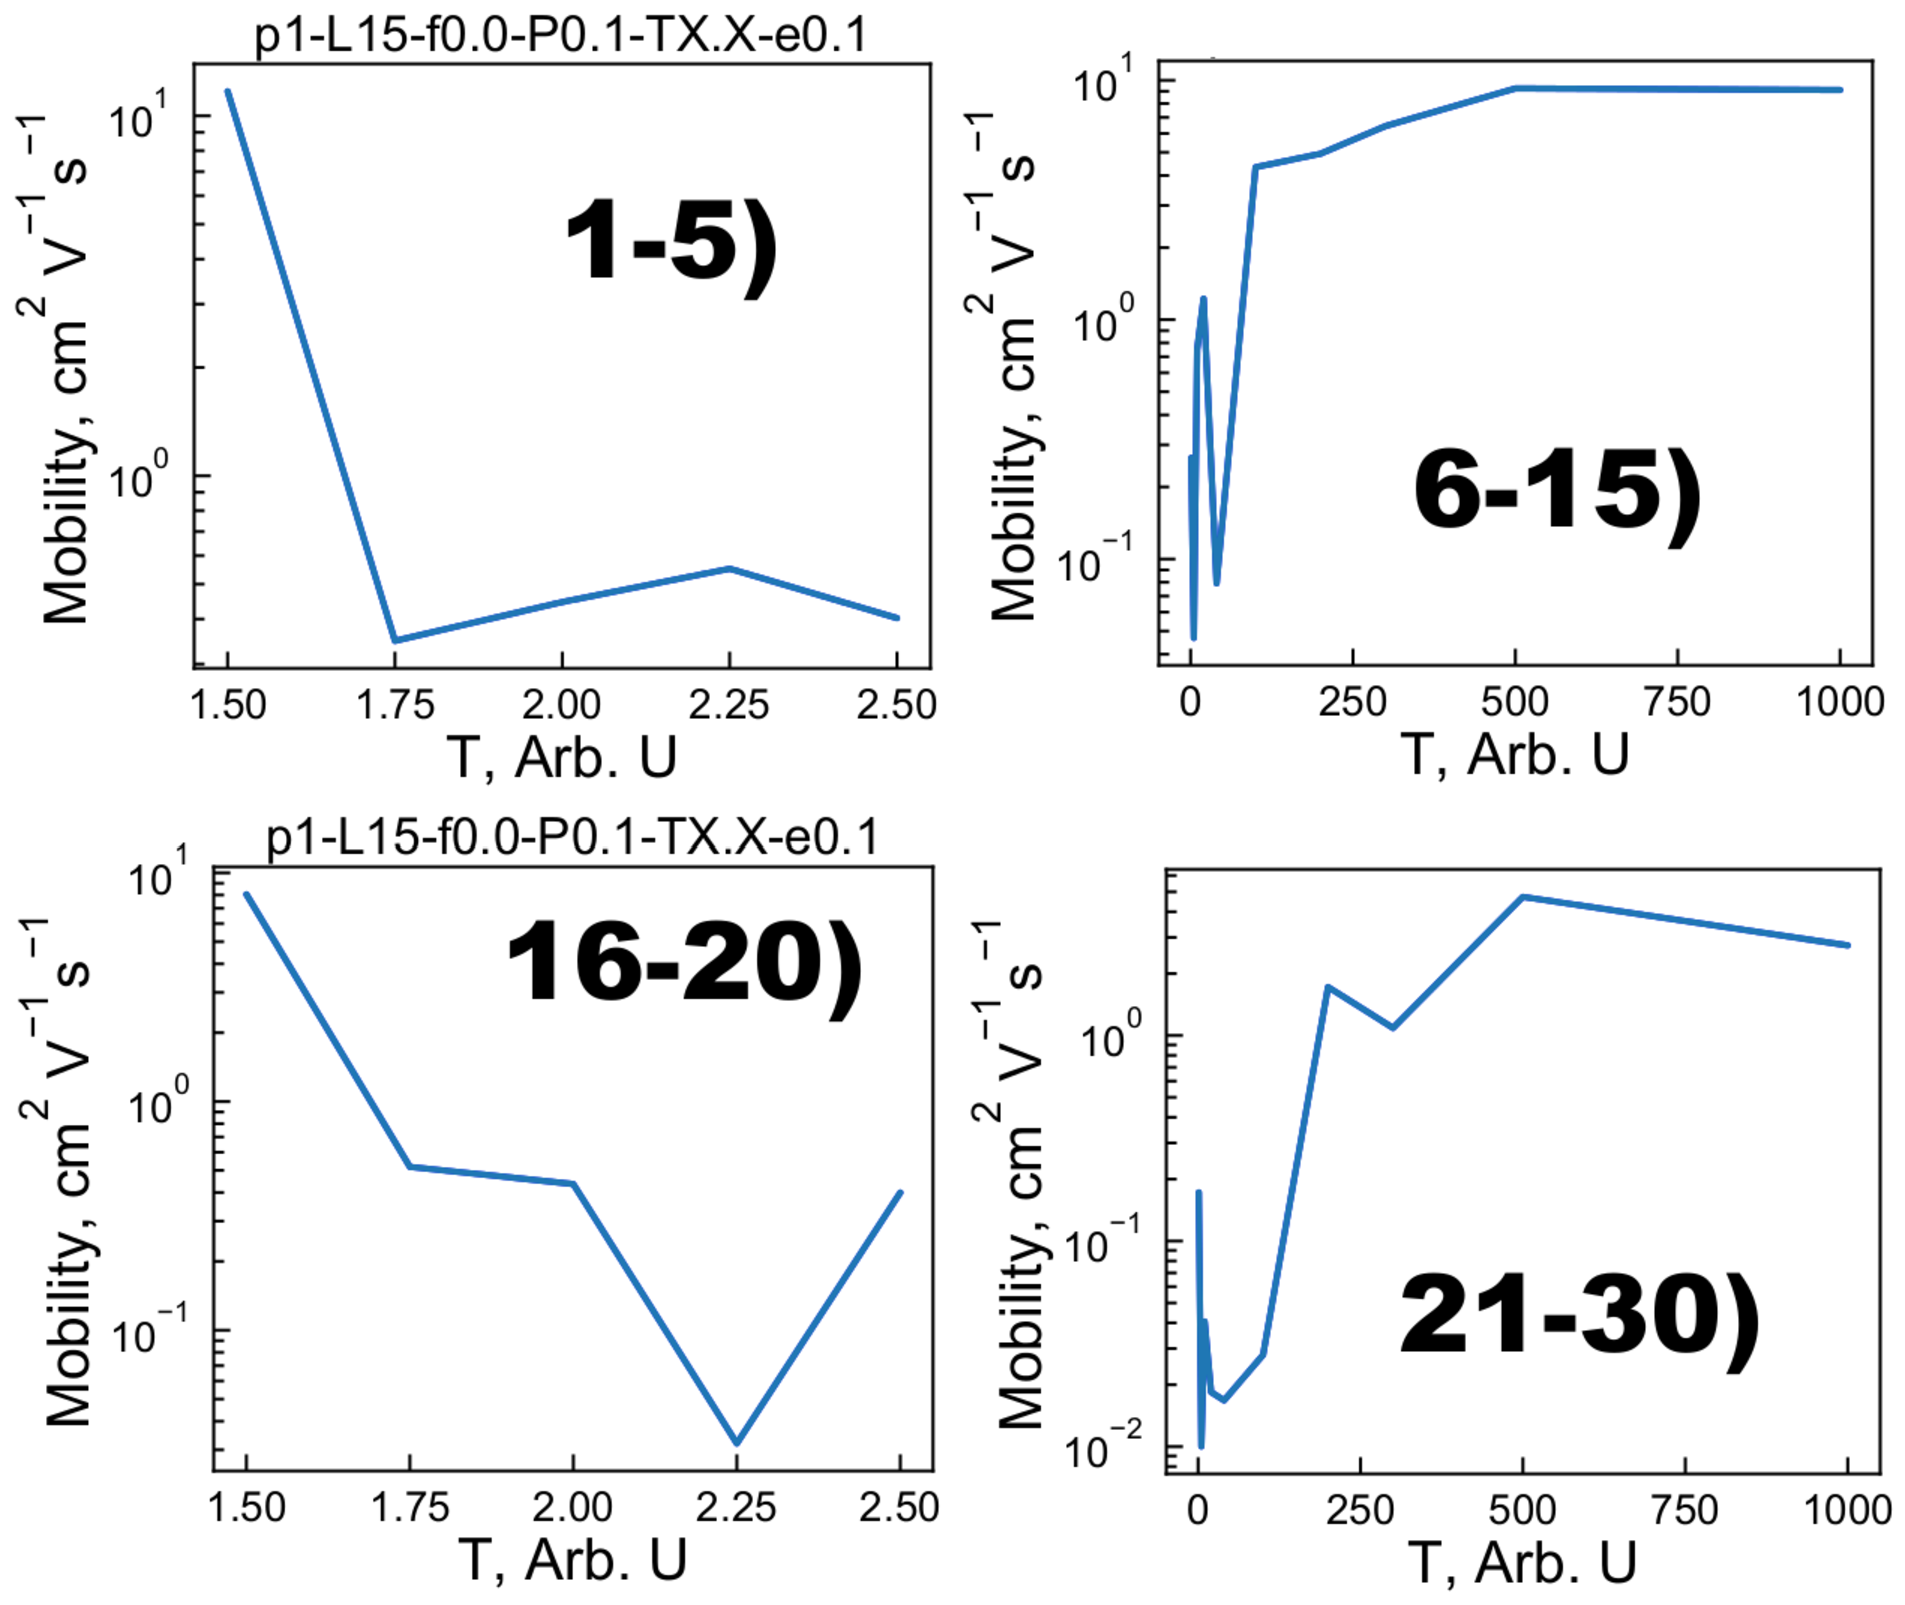
\includegraphics[width=\textwidth]{Figures/mobilityHole.pdf}
    \caption{The mobility trends observed over all jobs.}
	\label{fig:Mob}
\end{figure}

Representative Values From Literature:
\begin{itemize}
    \item{Density: \SI{1.10}{\gcm}\cite{Newbloom2012a}}
\item{Mobility: \SI{1E-5}{} - \SI{1E-3}{\mobunits}\cite{Ballantyne2008b,Mauer2010,Pandey2000,Kim2006}}
\end{itemize}

\clearpage

\subsection{3D Carrier Network}

\begin{figure}[h!]\centering
	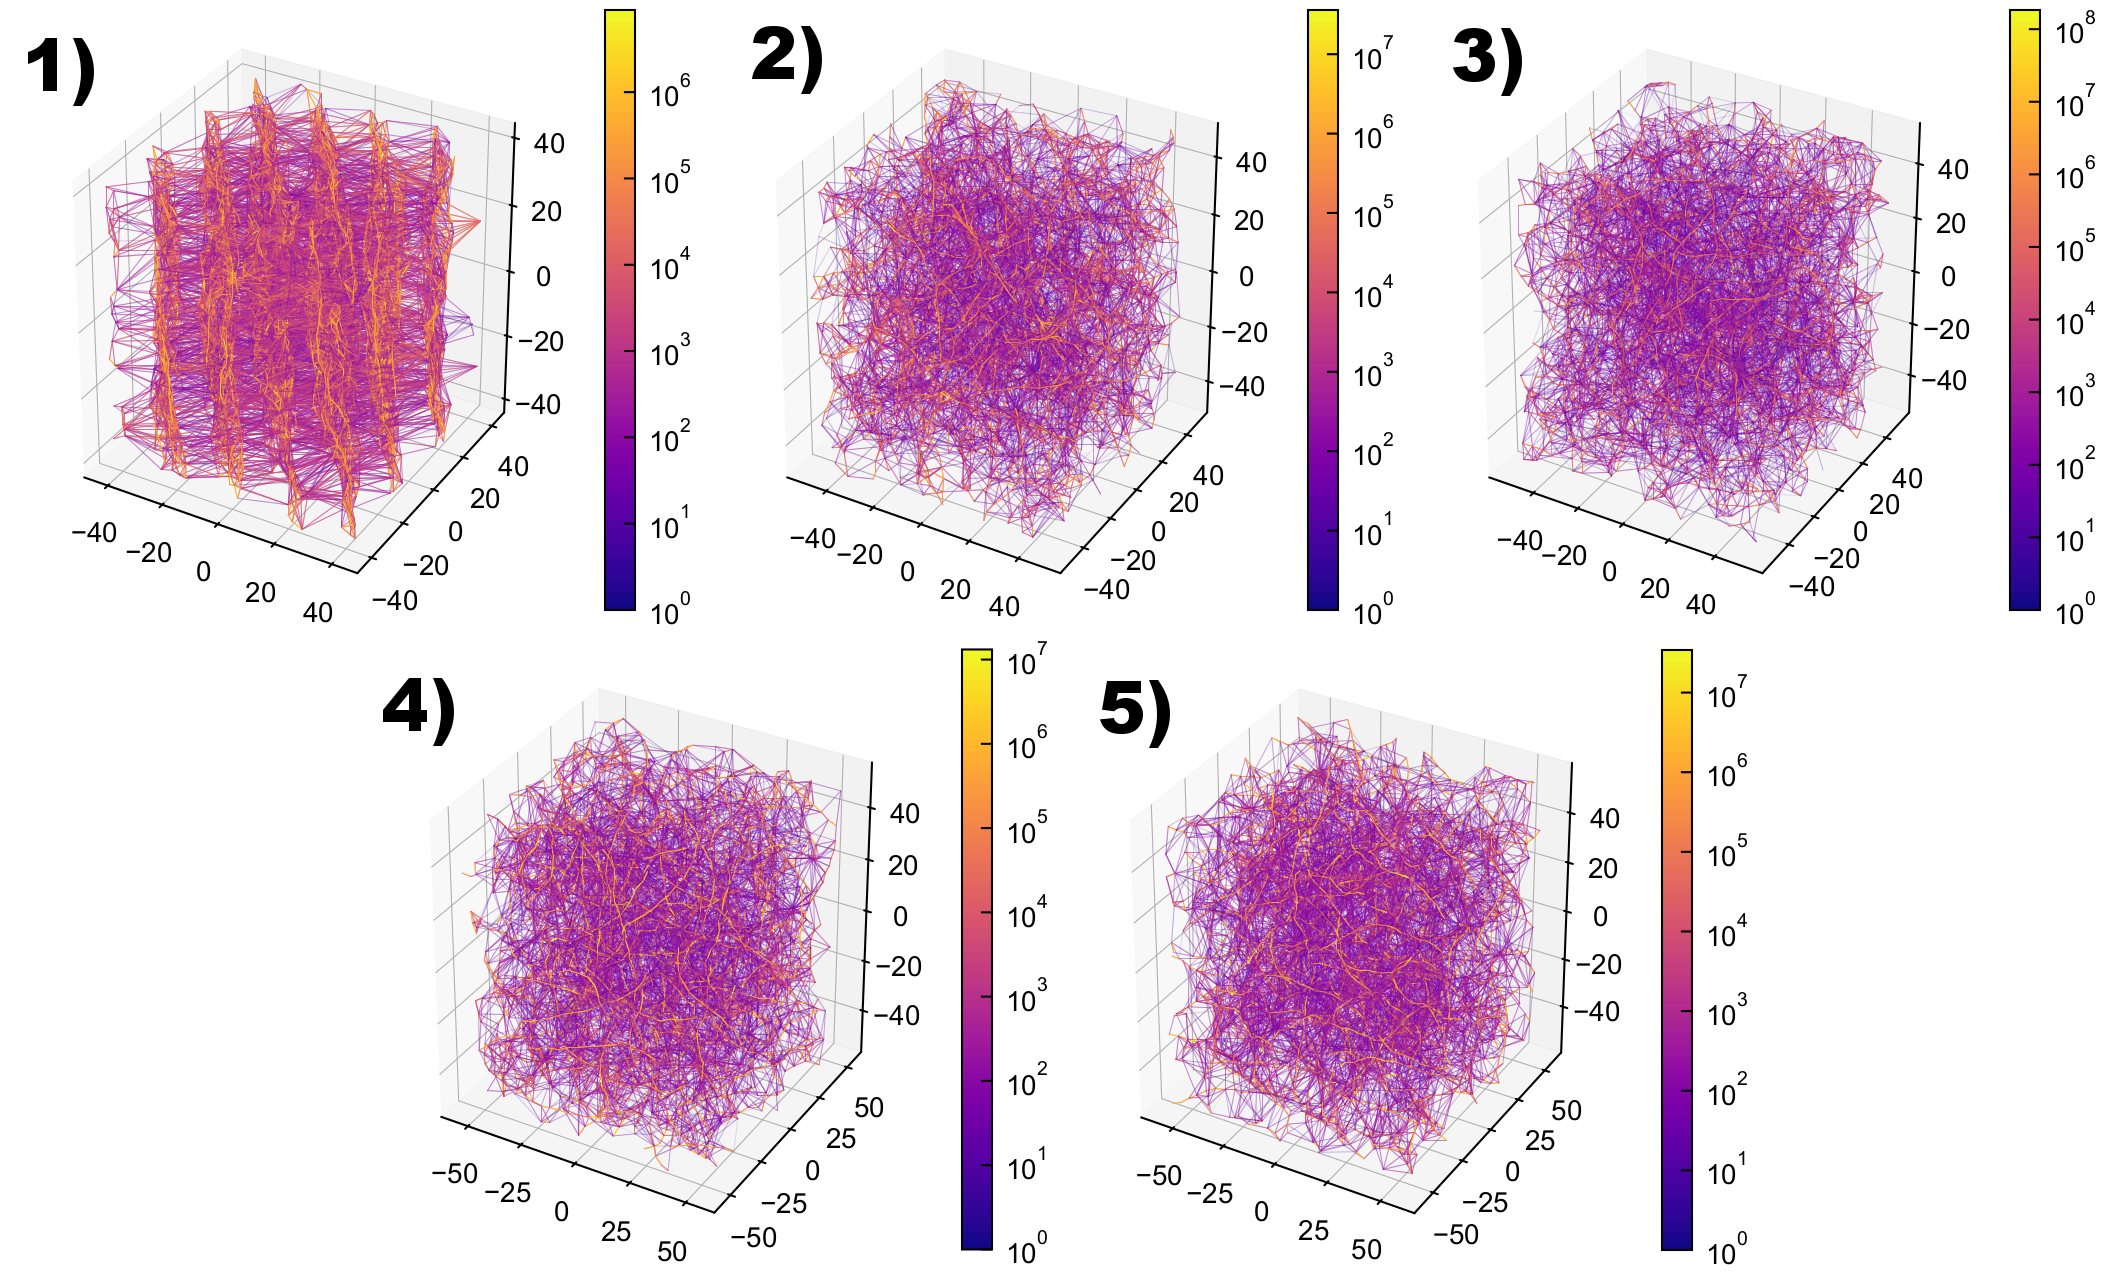
\includegraphics[width=\textwidth]{Figures/3dHole.png}
    \caption{The 3D heatmap of charge transport routes within the morphologies \textbf{1} - \textbf{5}.
    More yellow routes describe commonly accessed hops between pairs of chromophores, whereas more purple routes are less widely used in the KMC simulations.
    Each node therefore represents the location of a single chromophore.
The intensity value for the route is currently taken to be \texttt{I $=$ np.log10(freq) $/$ np.log10(max\_freq)}.}
	\label{fig:3dNetwork}
\end{figure}


\begin{figure}[h!]\centering
	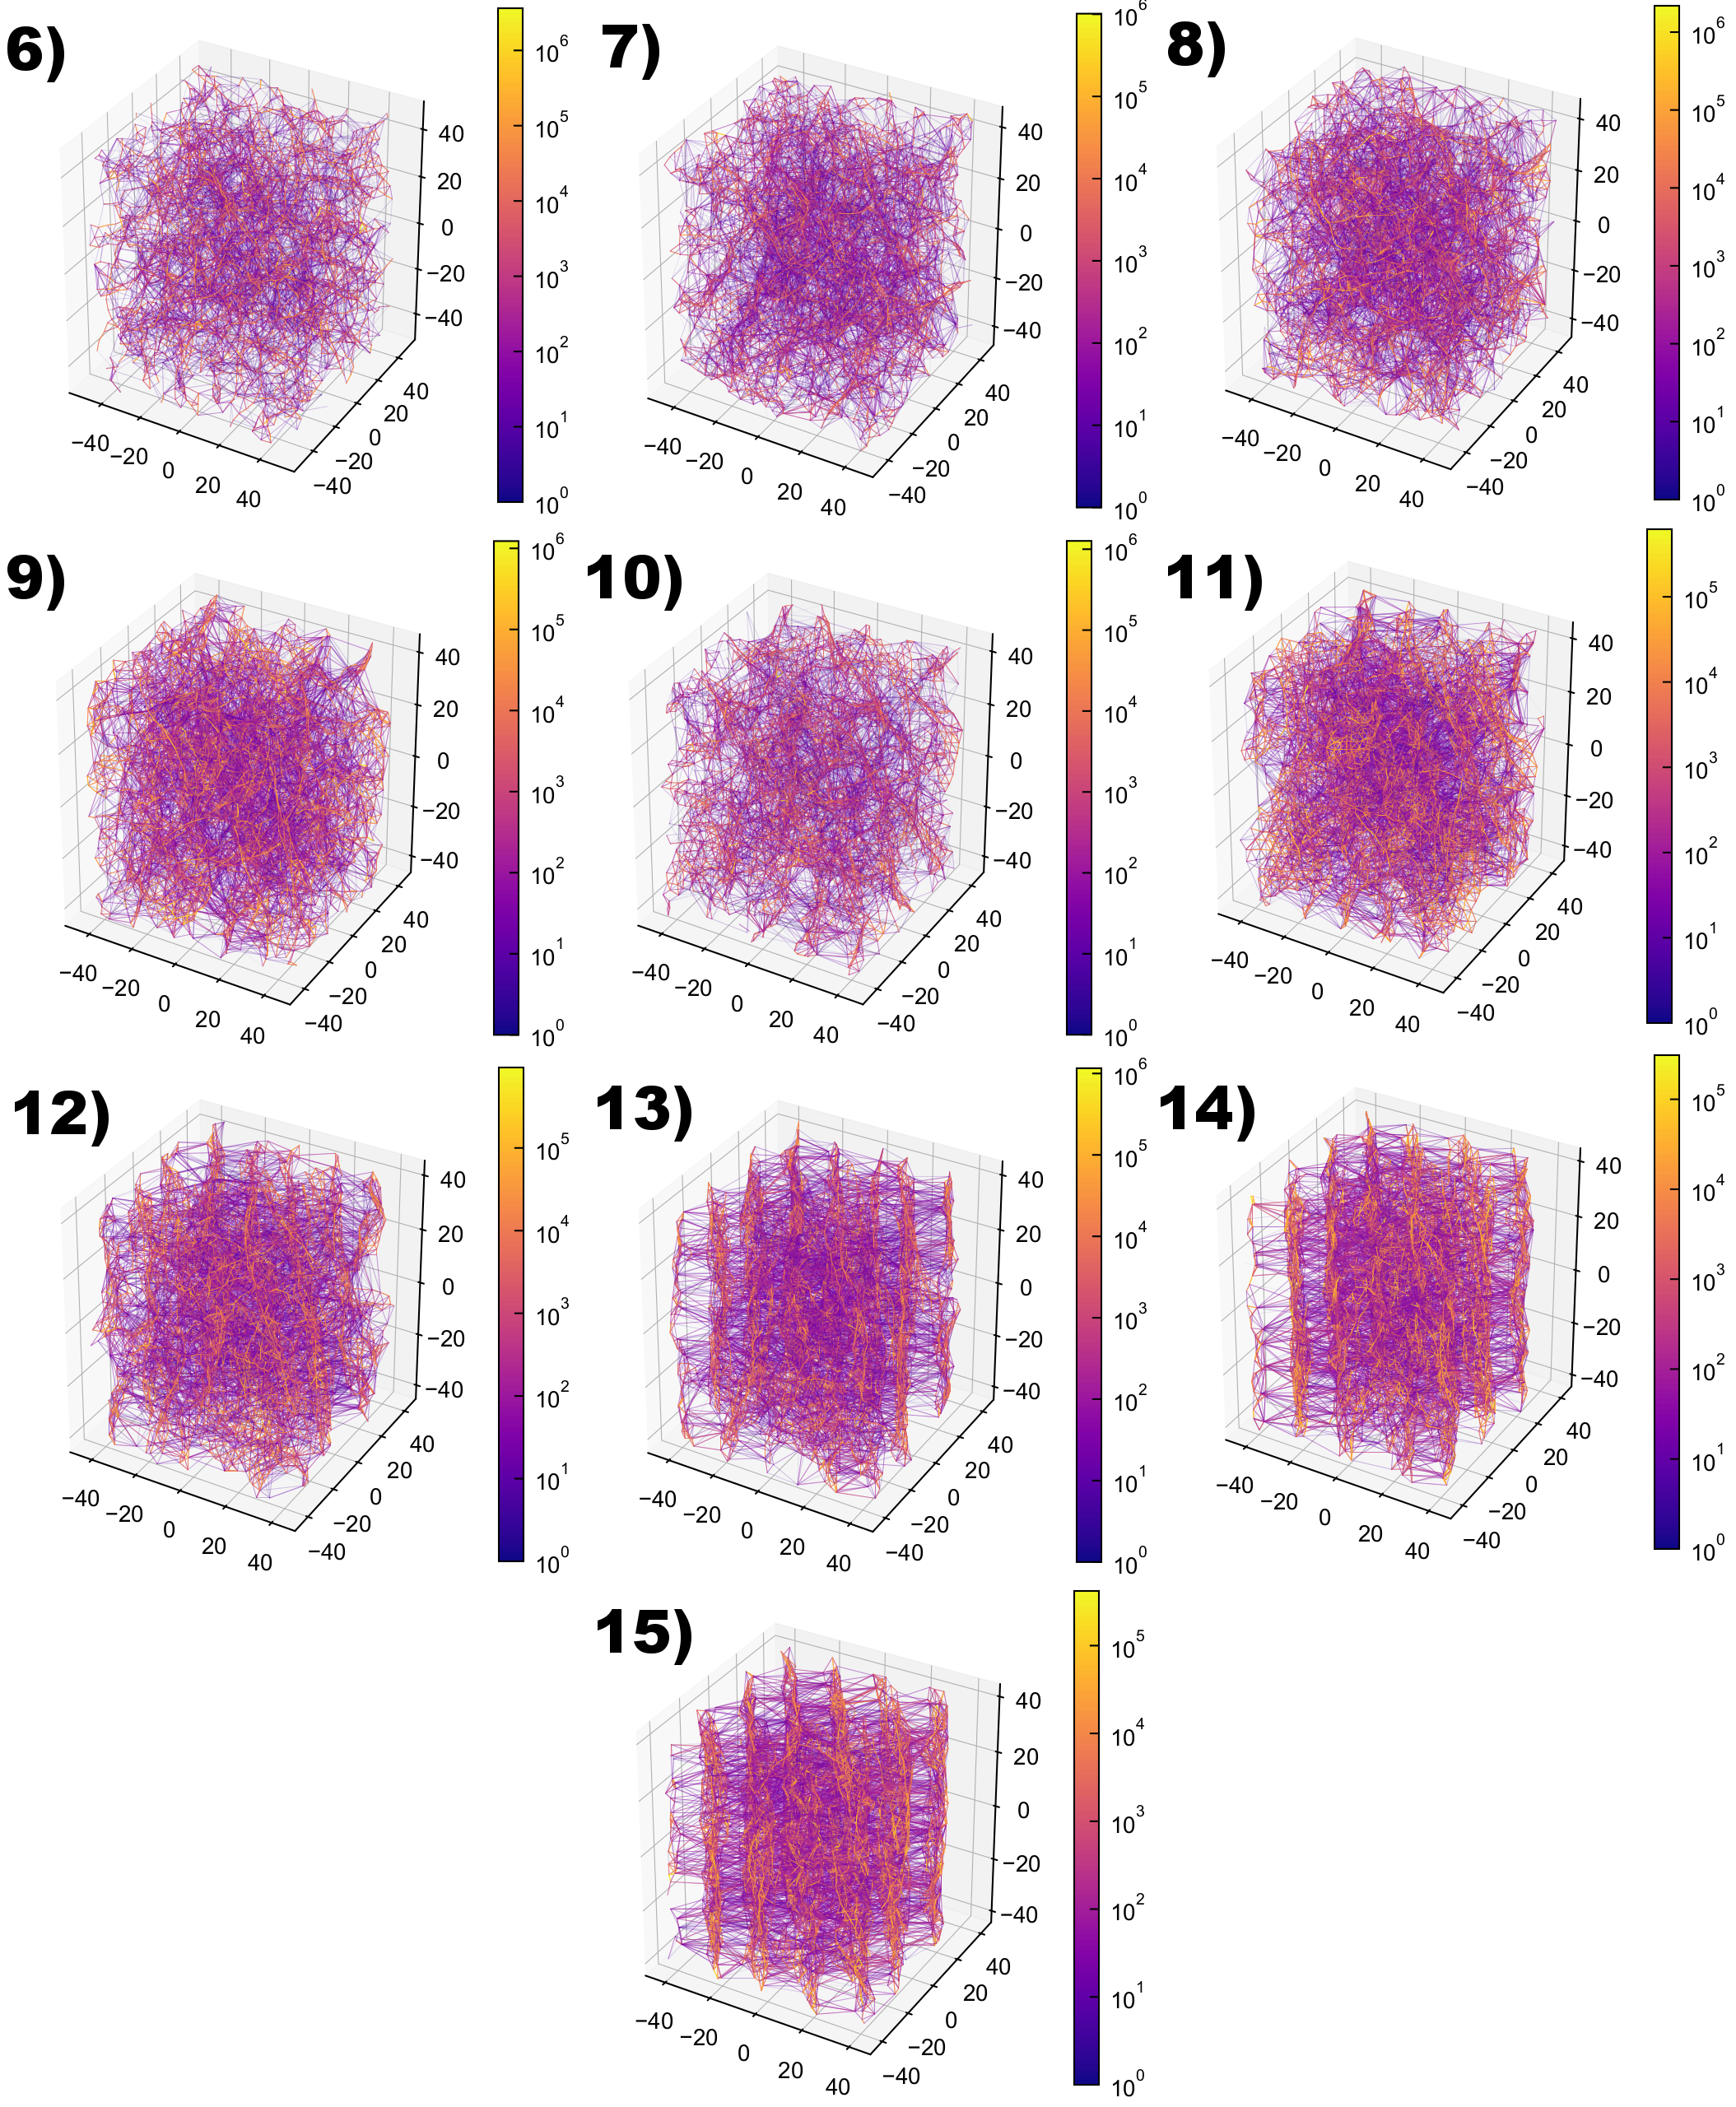
\includegraphics[width=\textwidth]{Figures/3dHoleFrame.png}
    \caption{The 3D heatmap of charge transport routes within the morphologies \textbf{6} - \textbf{15}.
    More yellow routes describe commonly accessed hops between pairs of chromophores, whereas more purple routes are less widely used in the KMC simulations.
    Each node therefore represents the location of a single chromophore.
The intensity value for the route is currently taken to be \texttt{I $=$ np.log10(freq) $/$ np.log10(max\_freq)}.}
	\label{fig:3dNetworkFrame}
\end{figure}


\begin{figure}[h!]\centering
	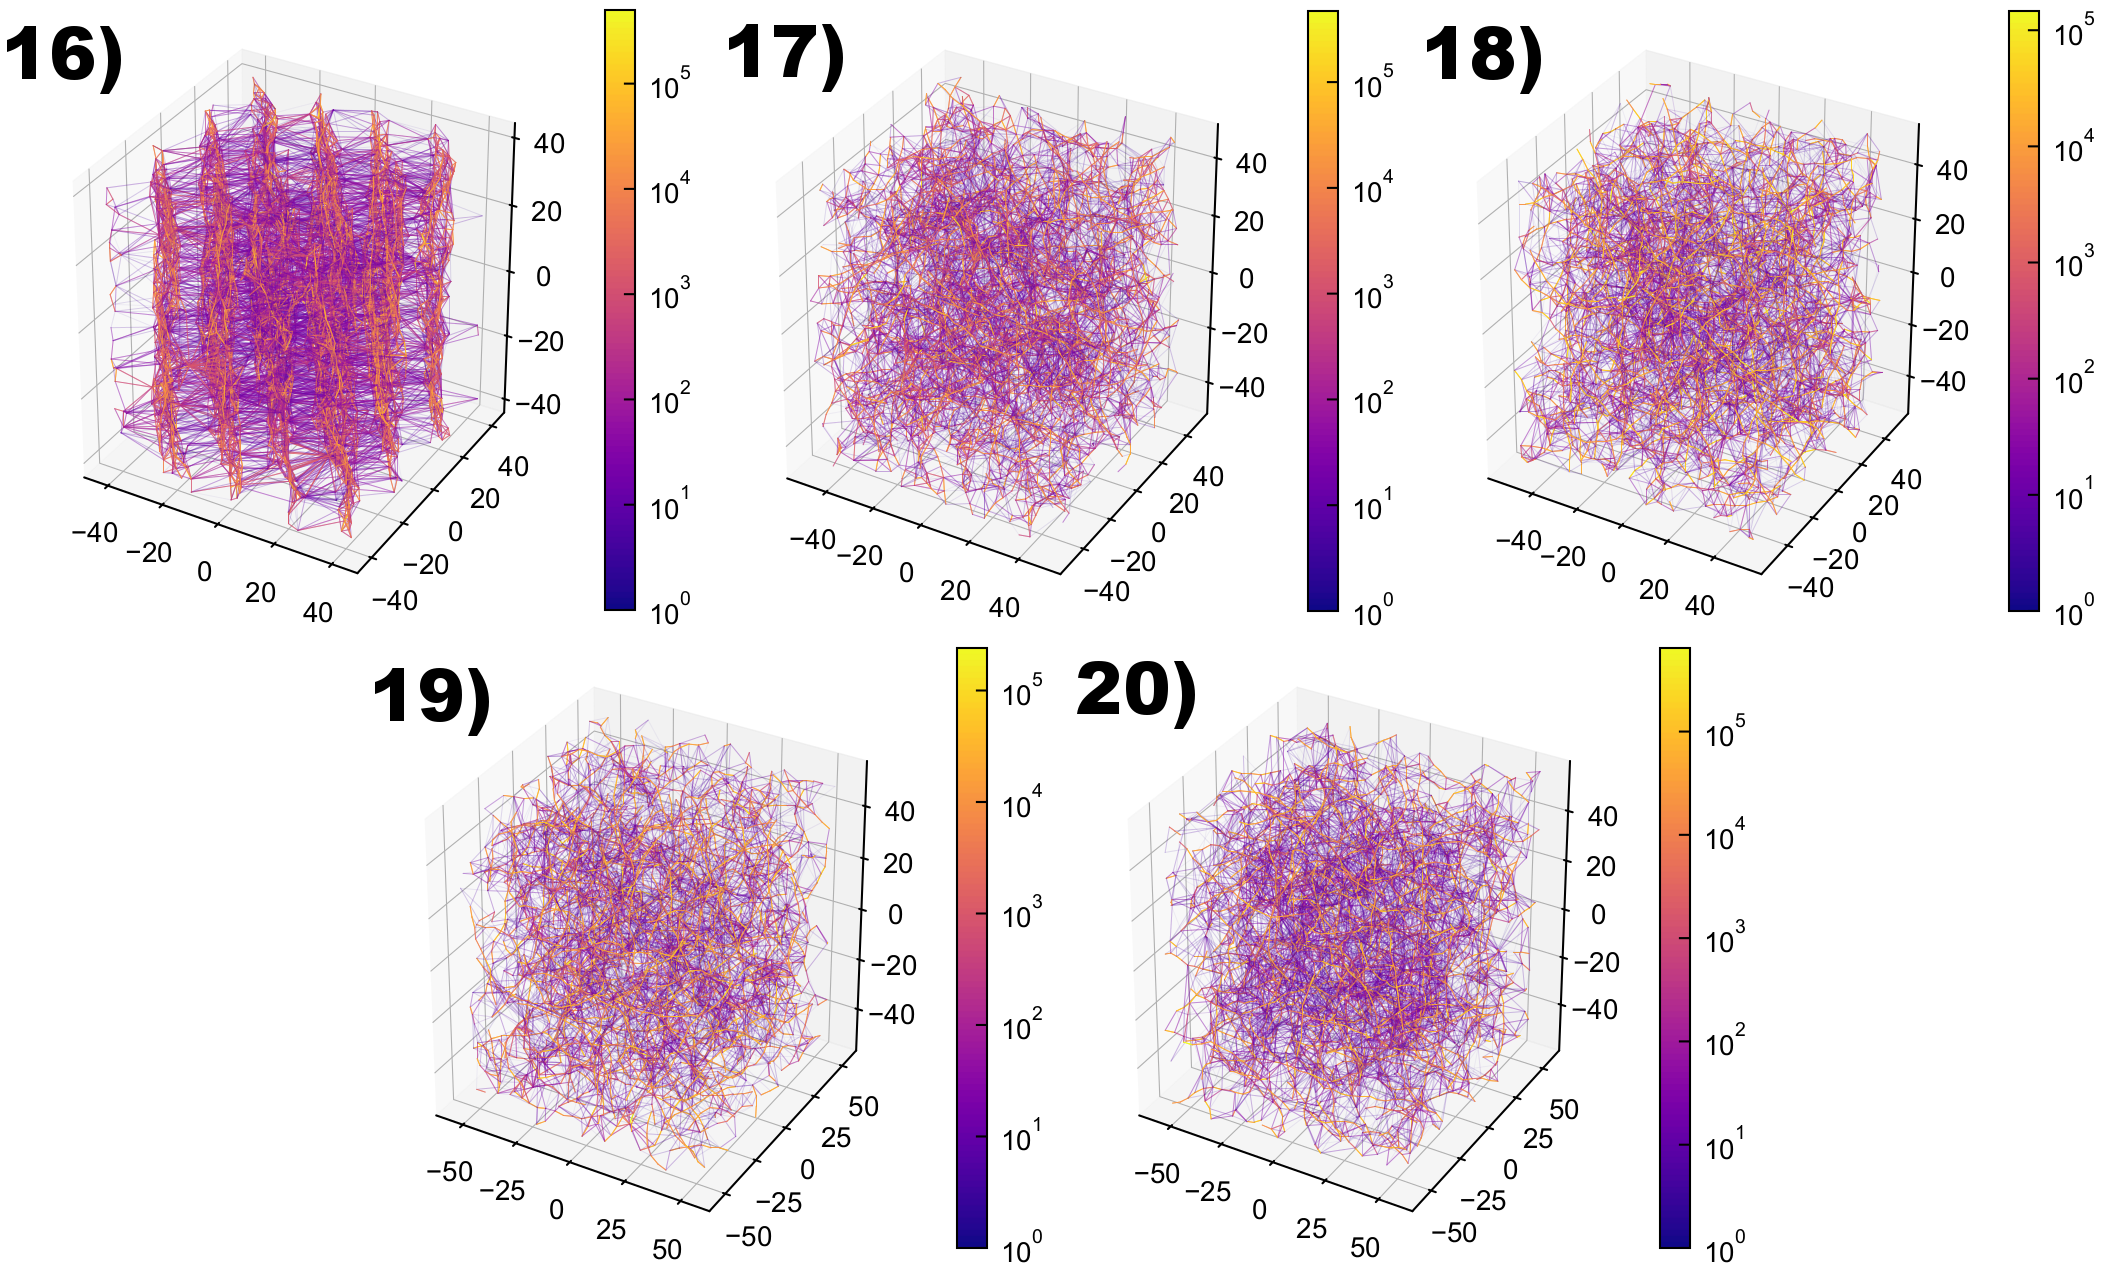
\includegraphics[width=\textwidth]{Figures/3dHoleOrig.png}
    \caption{The 3D heatmap of charge transport routes within the morphologies \textbf{16} - \textbf{20}.
    More yellow routes describe commonly accessed hops between pairs of chromophores, whereas more purple routes are less widely used in the KMC simulations.
    Each node therefore represents the location of a single chromophore.
The intensity value for the route is currently taken to be \texttt{I $=$ np.log10(freq) $/$ np.log10(max\_freq)}.}
	\label{fig:3dNetworkOrig}
\end{figure}


\begin{figure}[h!]\centering
	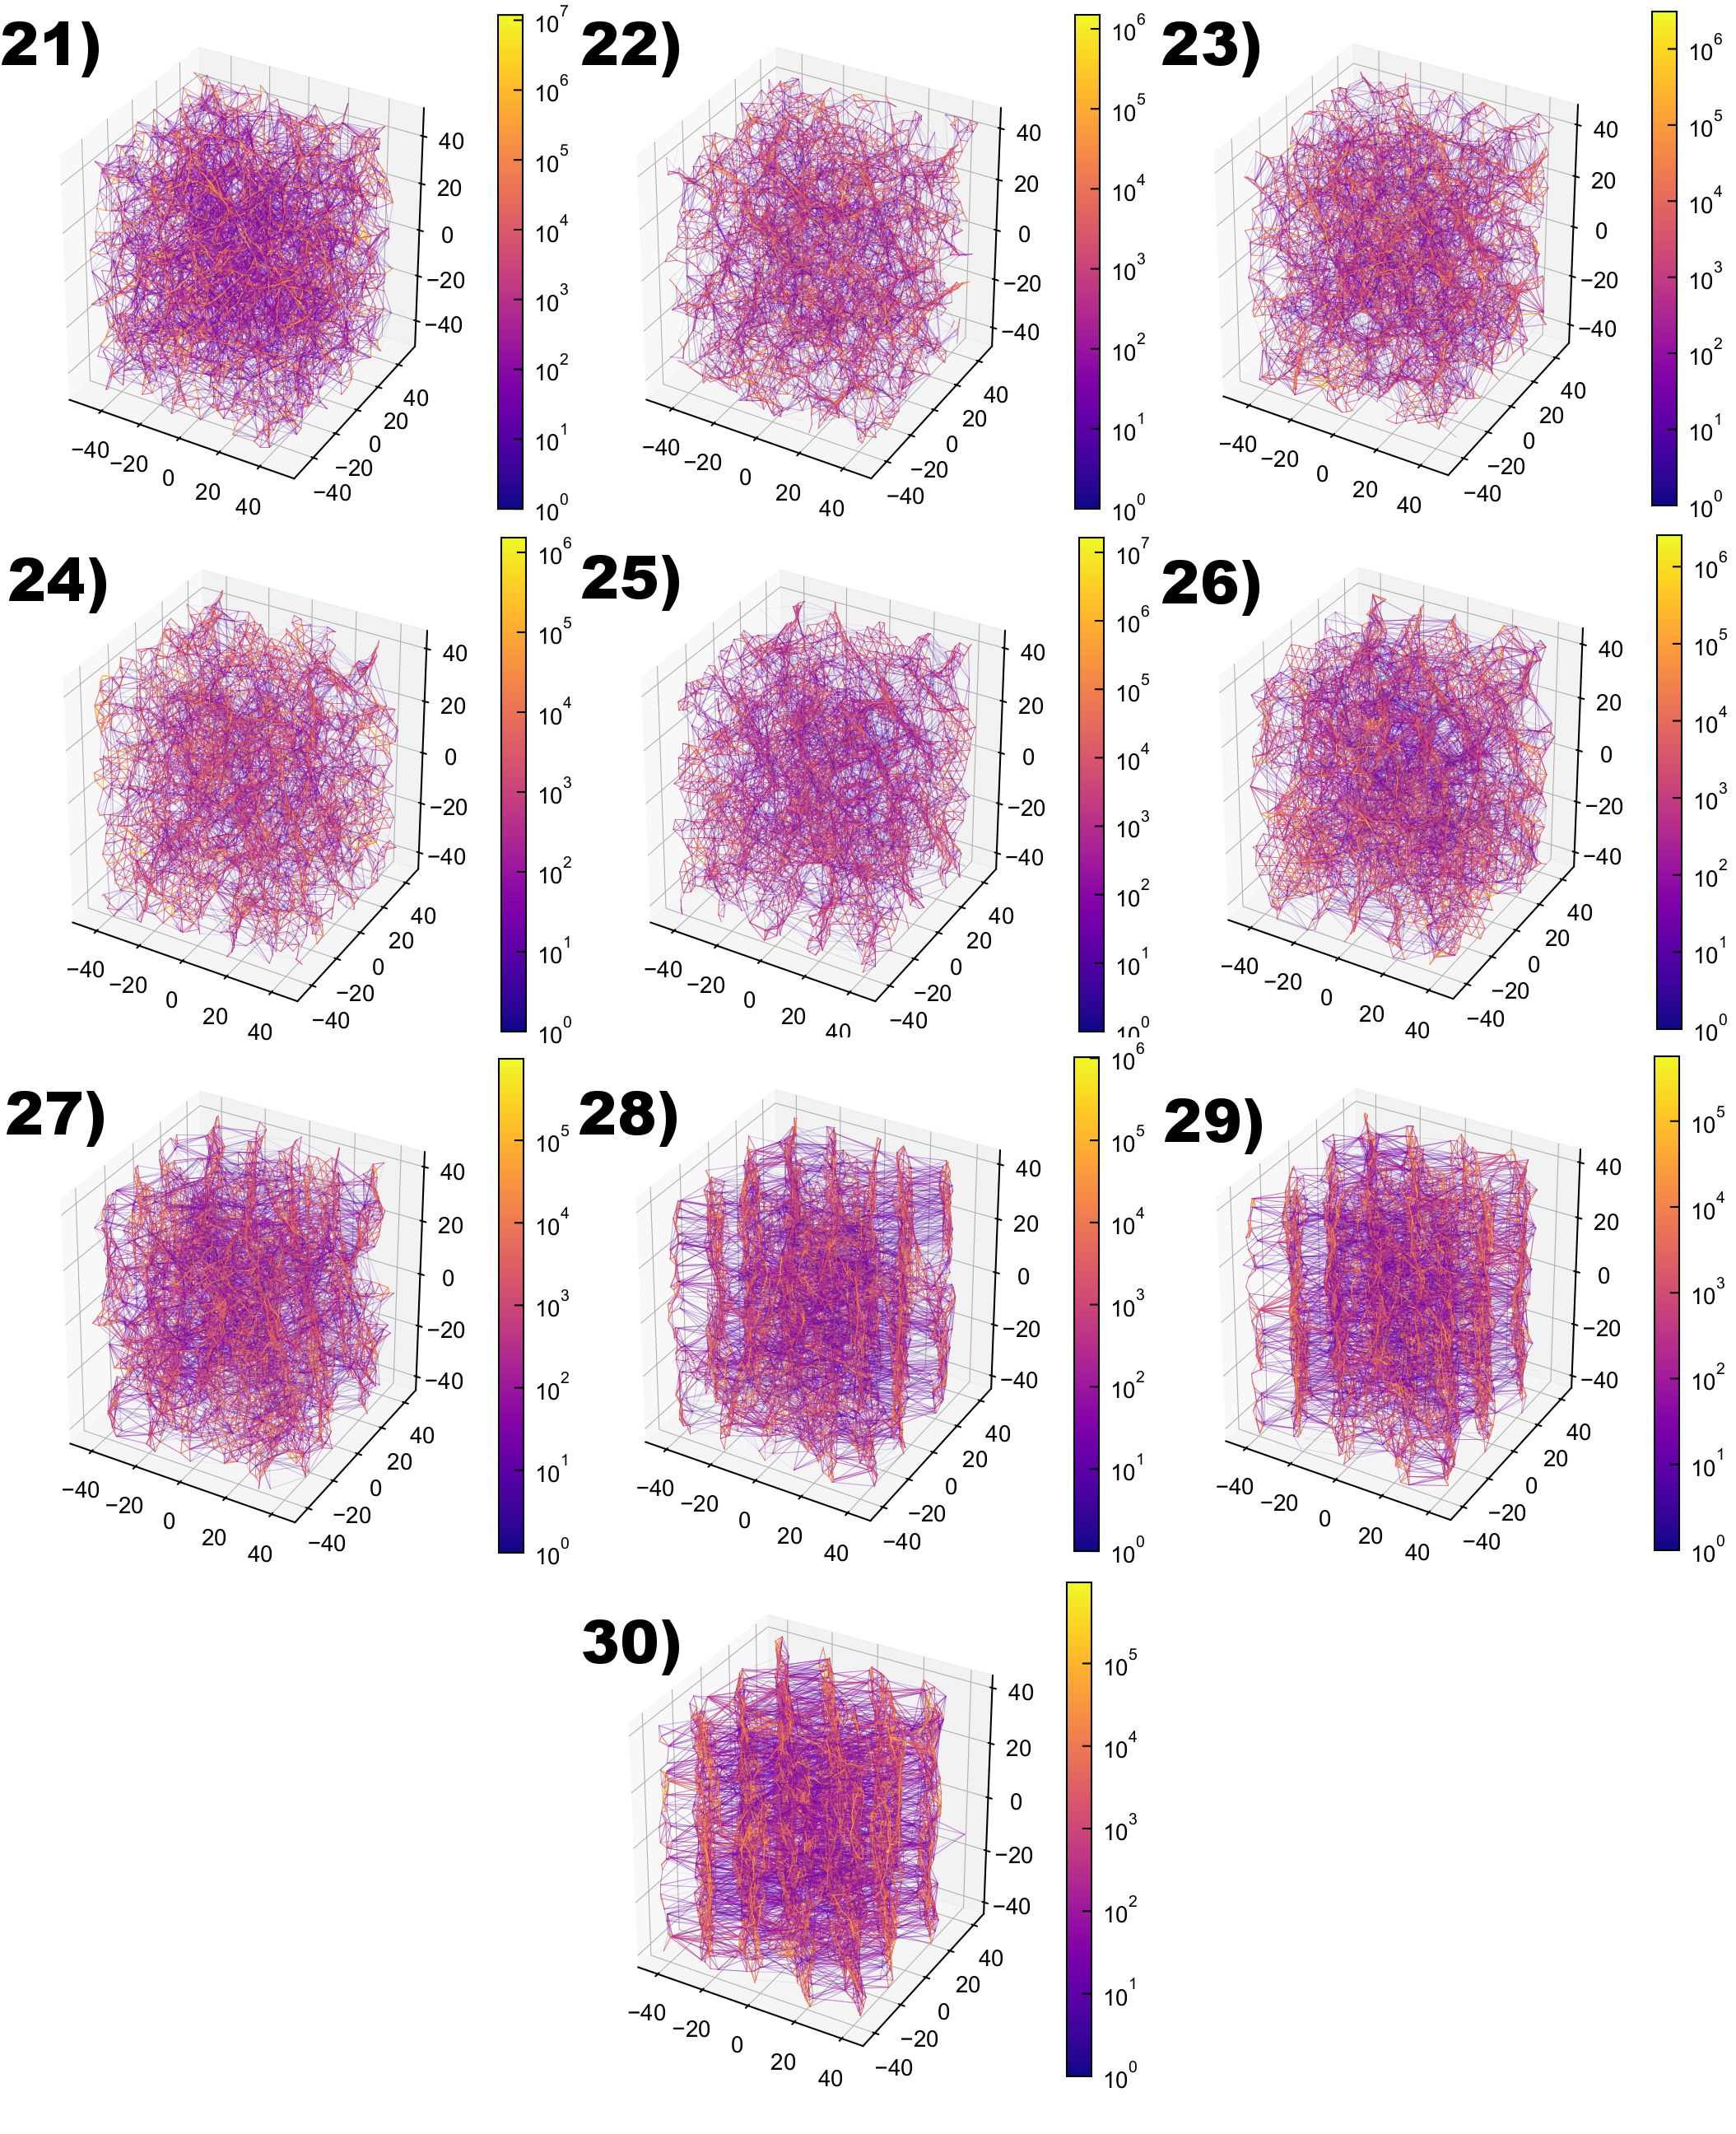
\includegraphics[width=\textwidth]{Figures/3dHoleFrameOrig.png}
    \caption{The 3D heatmap of charge transport routes within the morphologies \textbf{21} - \textbf{30}.
    More yellow routes describe commonly accessed hops between pairs of chromophores, whereas more purple routes are less widely used in the KMC simulations.
    Each node therefore represents the location of a single chromophore.
The intensity value for the route is currently taken to be \texttt{I $=$ np.log10(freq) $/$ np.log10(max\_freq)}.}
	\label{fig:3dNetworkFrameOrig}
\end{figure}

\clearpage
\subsection{Anisotropies}


\begin{figure}[h!]\centering
	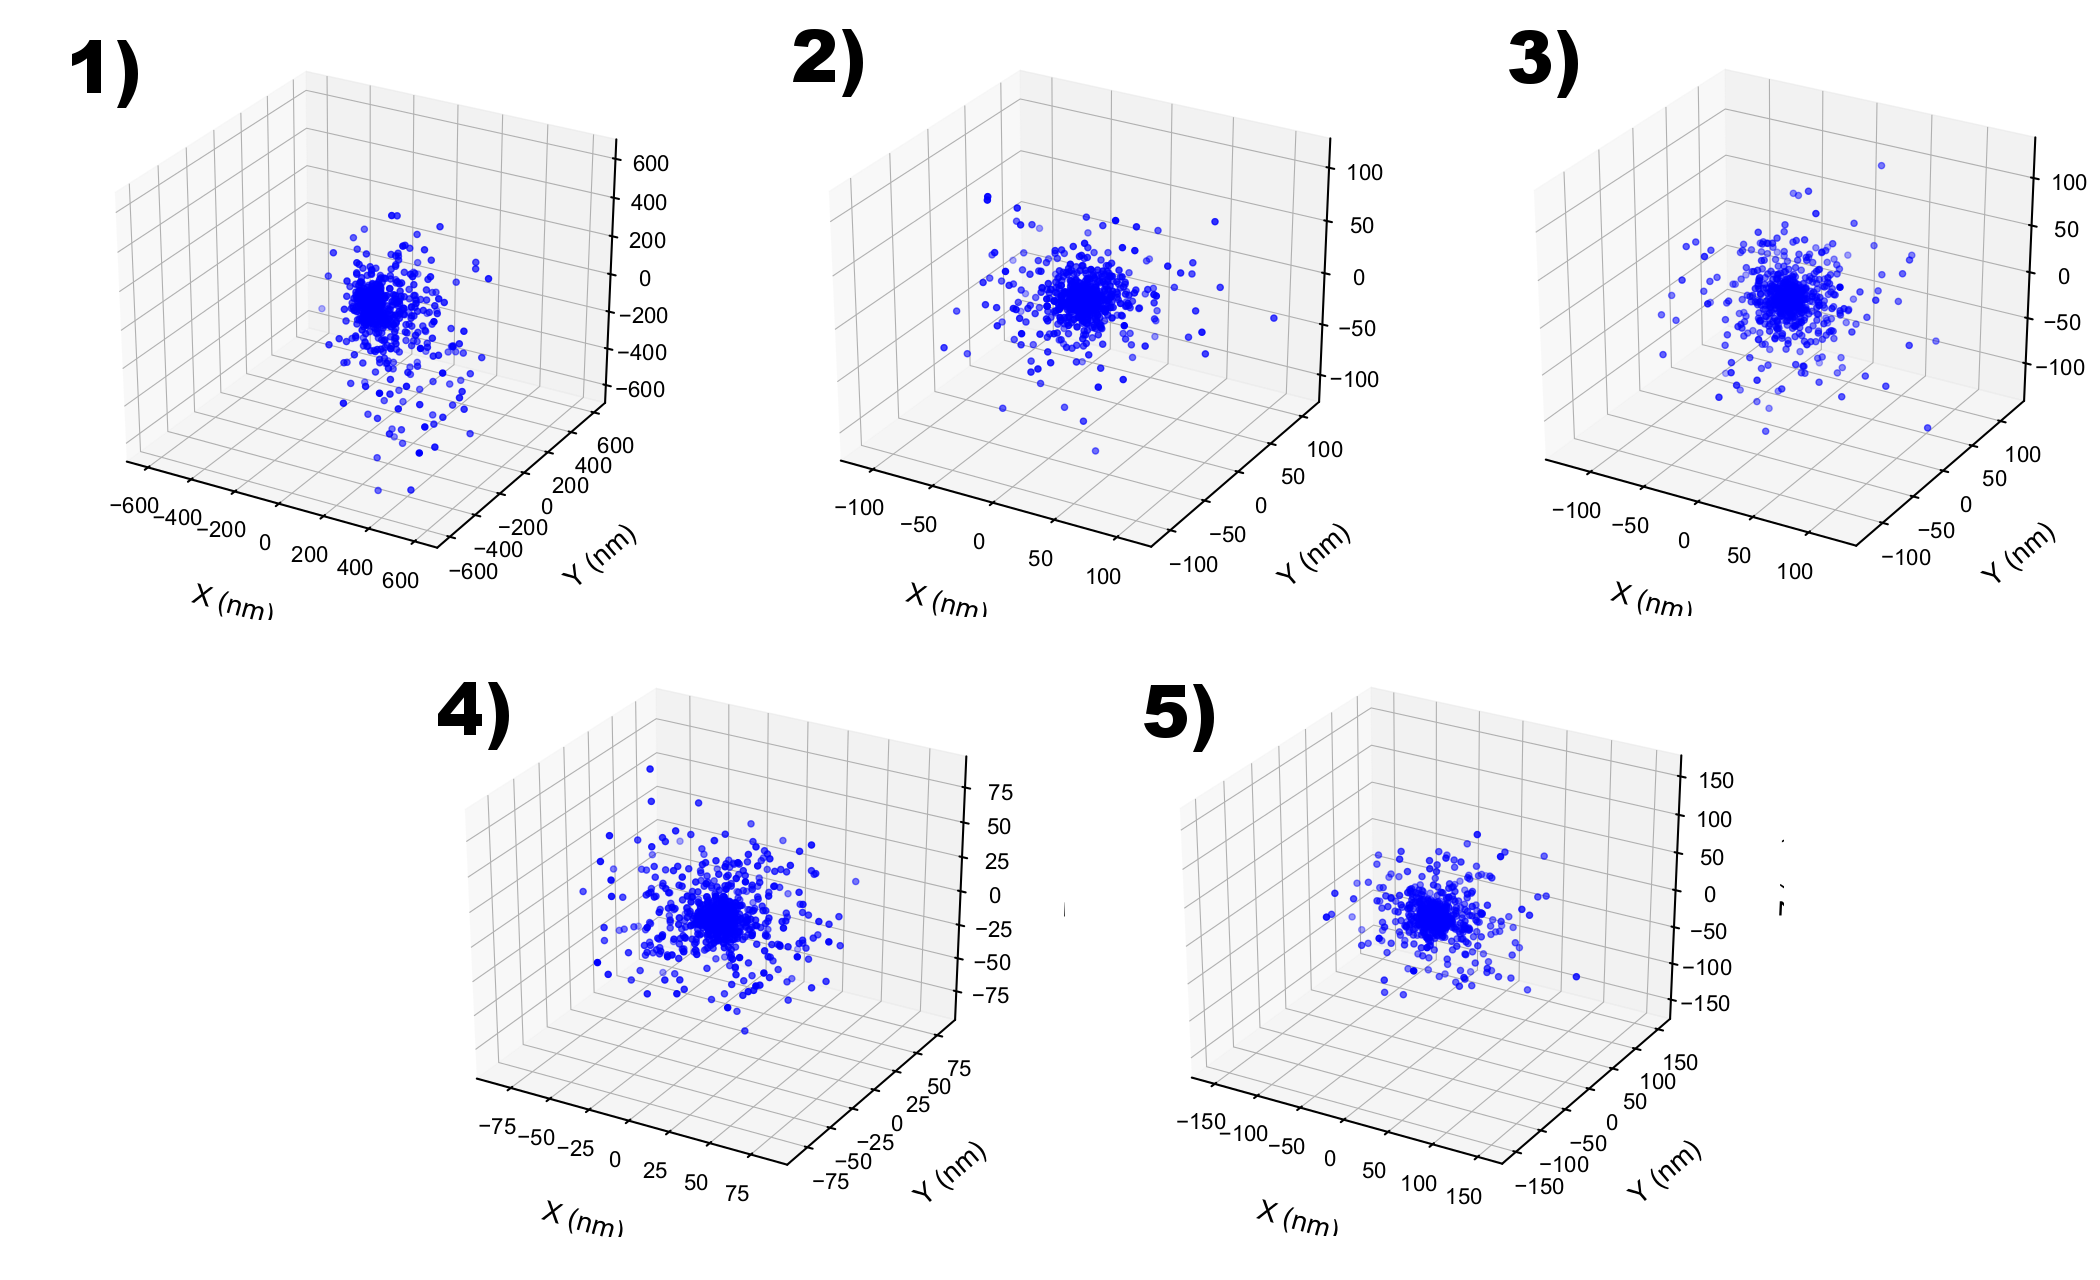
\includegraphics[width=\textwidth]{Figures/anisotropyHole.png}
    \caption{The periodic anisotropies of the carrier transport within the morphologies \textbf{1} - \textbf{5}.}
	\label{fig:Anis}
\end{figure}

\begin{figure}[h!]\centering
	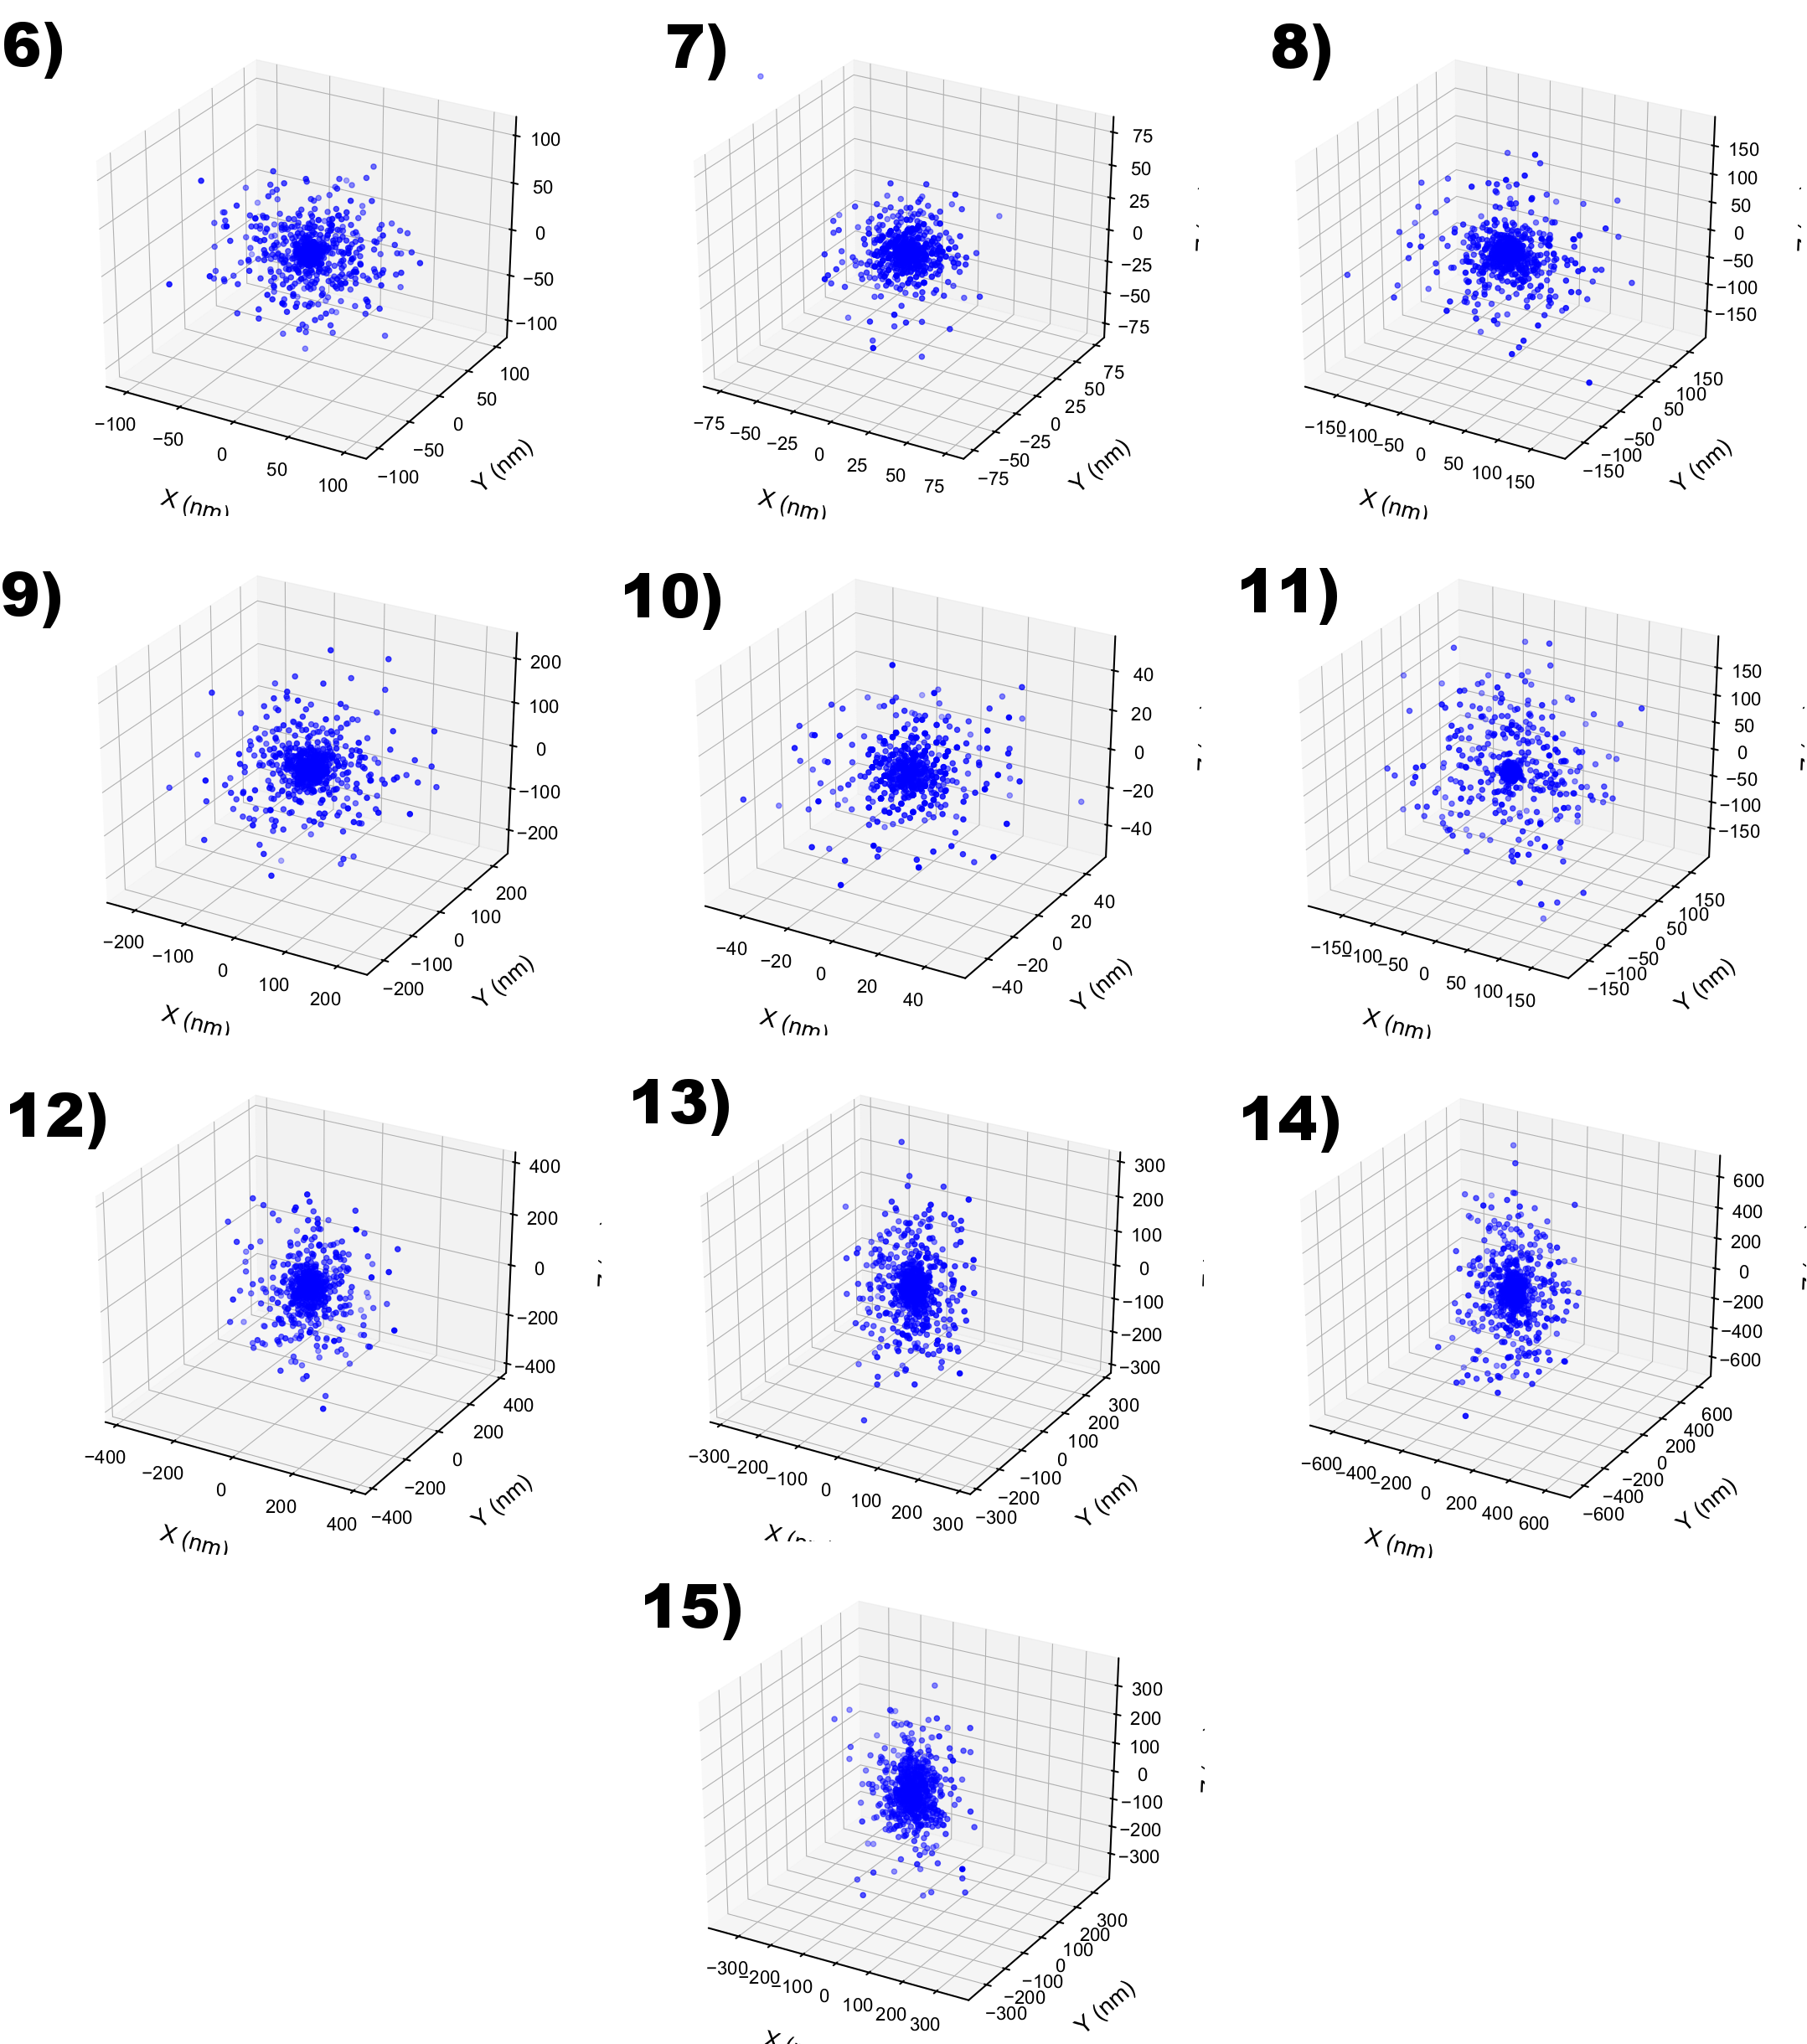
\includegraphics[width=\textwidth]{Figures/anisotropyHoleFrame.png}
    \caption{The periodic anisotropies of the carrier transport within the morphologies \textbf{6} - \textbf{15}.}
	\label{fig:AnisFrame}
\end{figure}


\begin{figure}[h!]\centering
	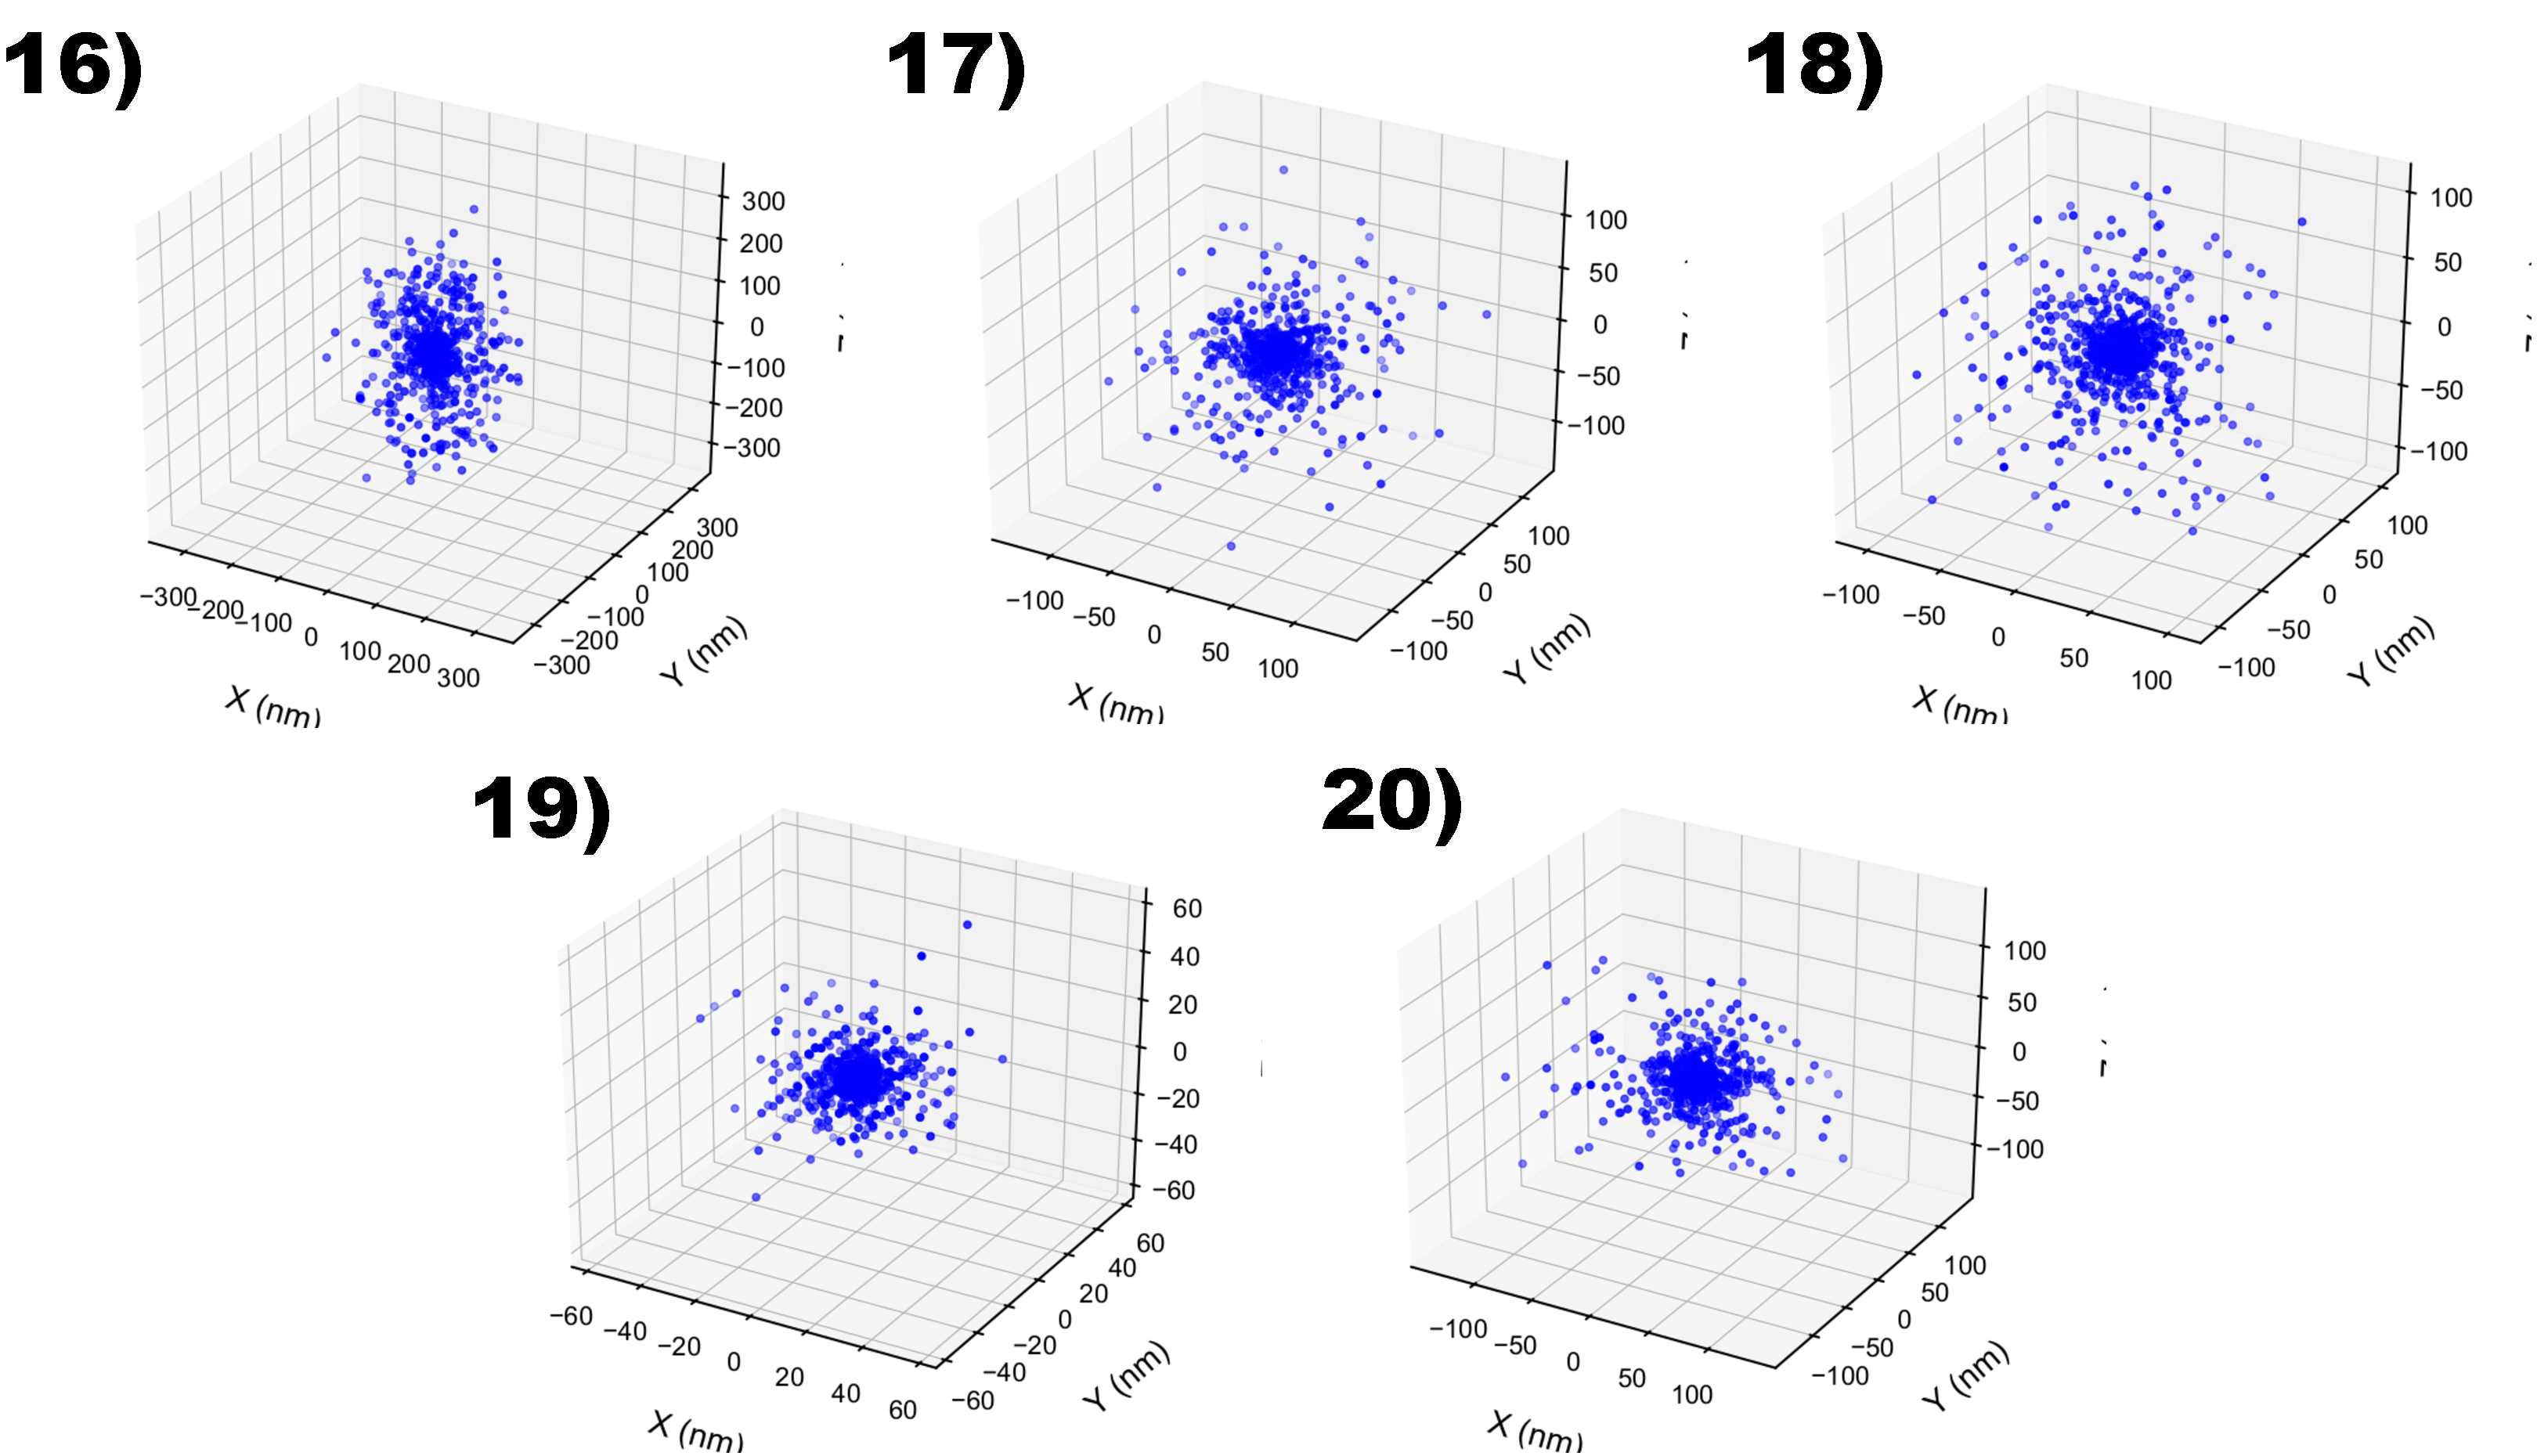
\includegraphics[width=\textwidth]{Figures/anisotropyHoleOrig.pdf}
    \caption{The periodic anisotropies of the carrier transport within the morphologies \textbf{16} - \textbf{20}.}
	\label{fig:AnisOrig}
\end{figure}

\begin{figure}[h!]\centering
	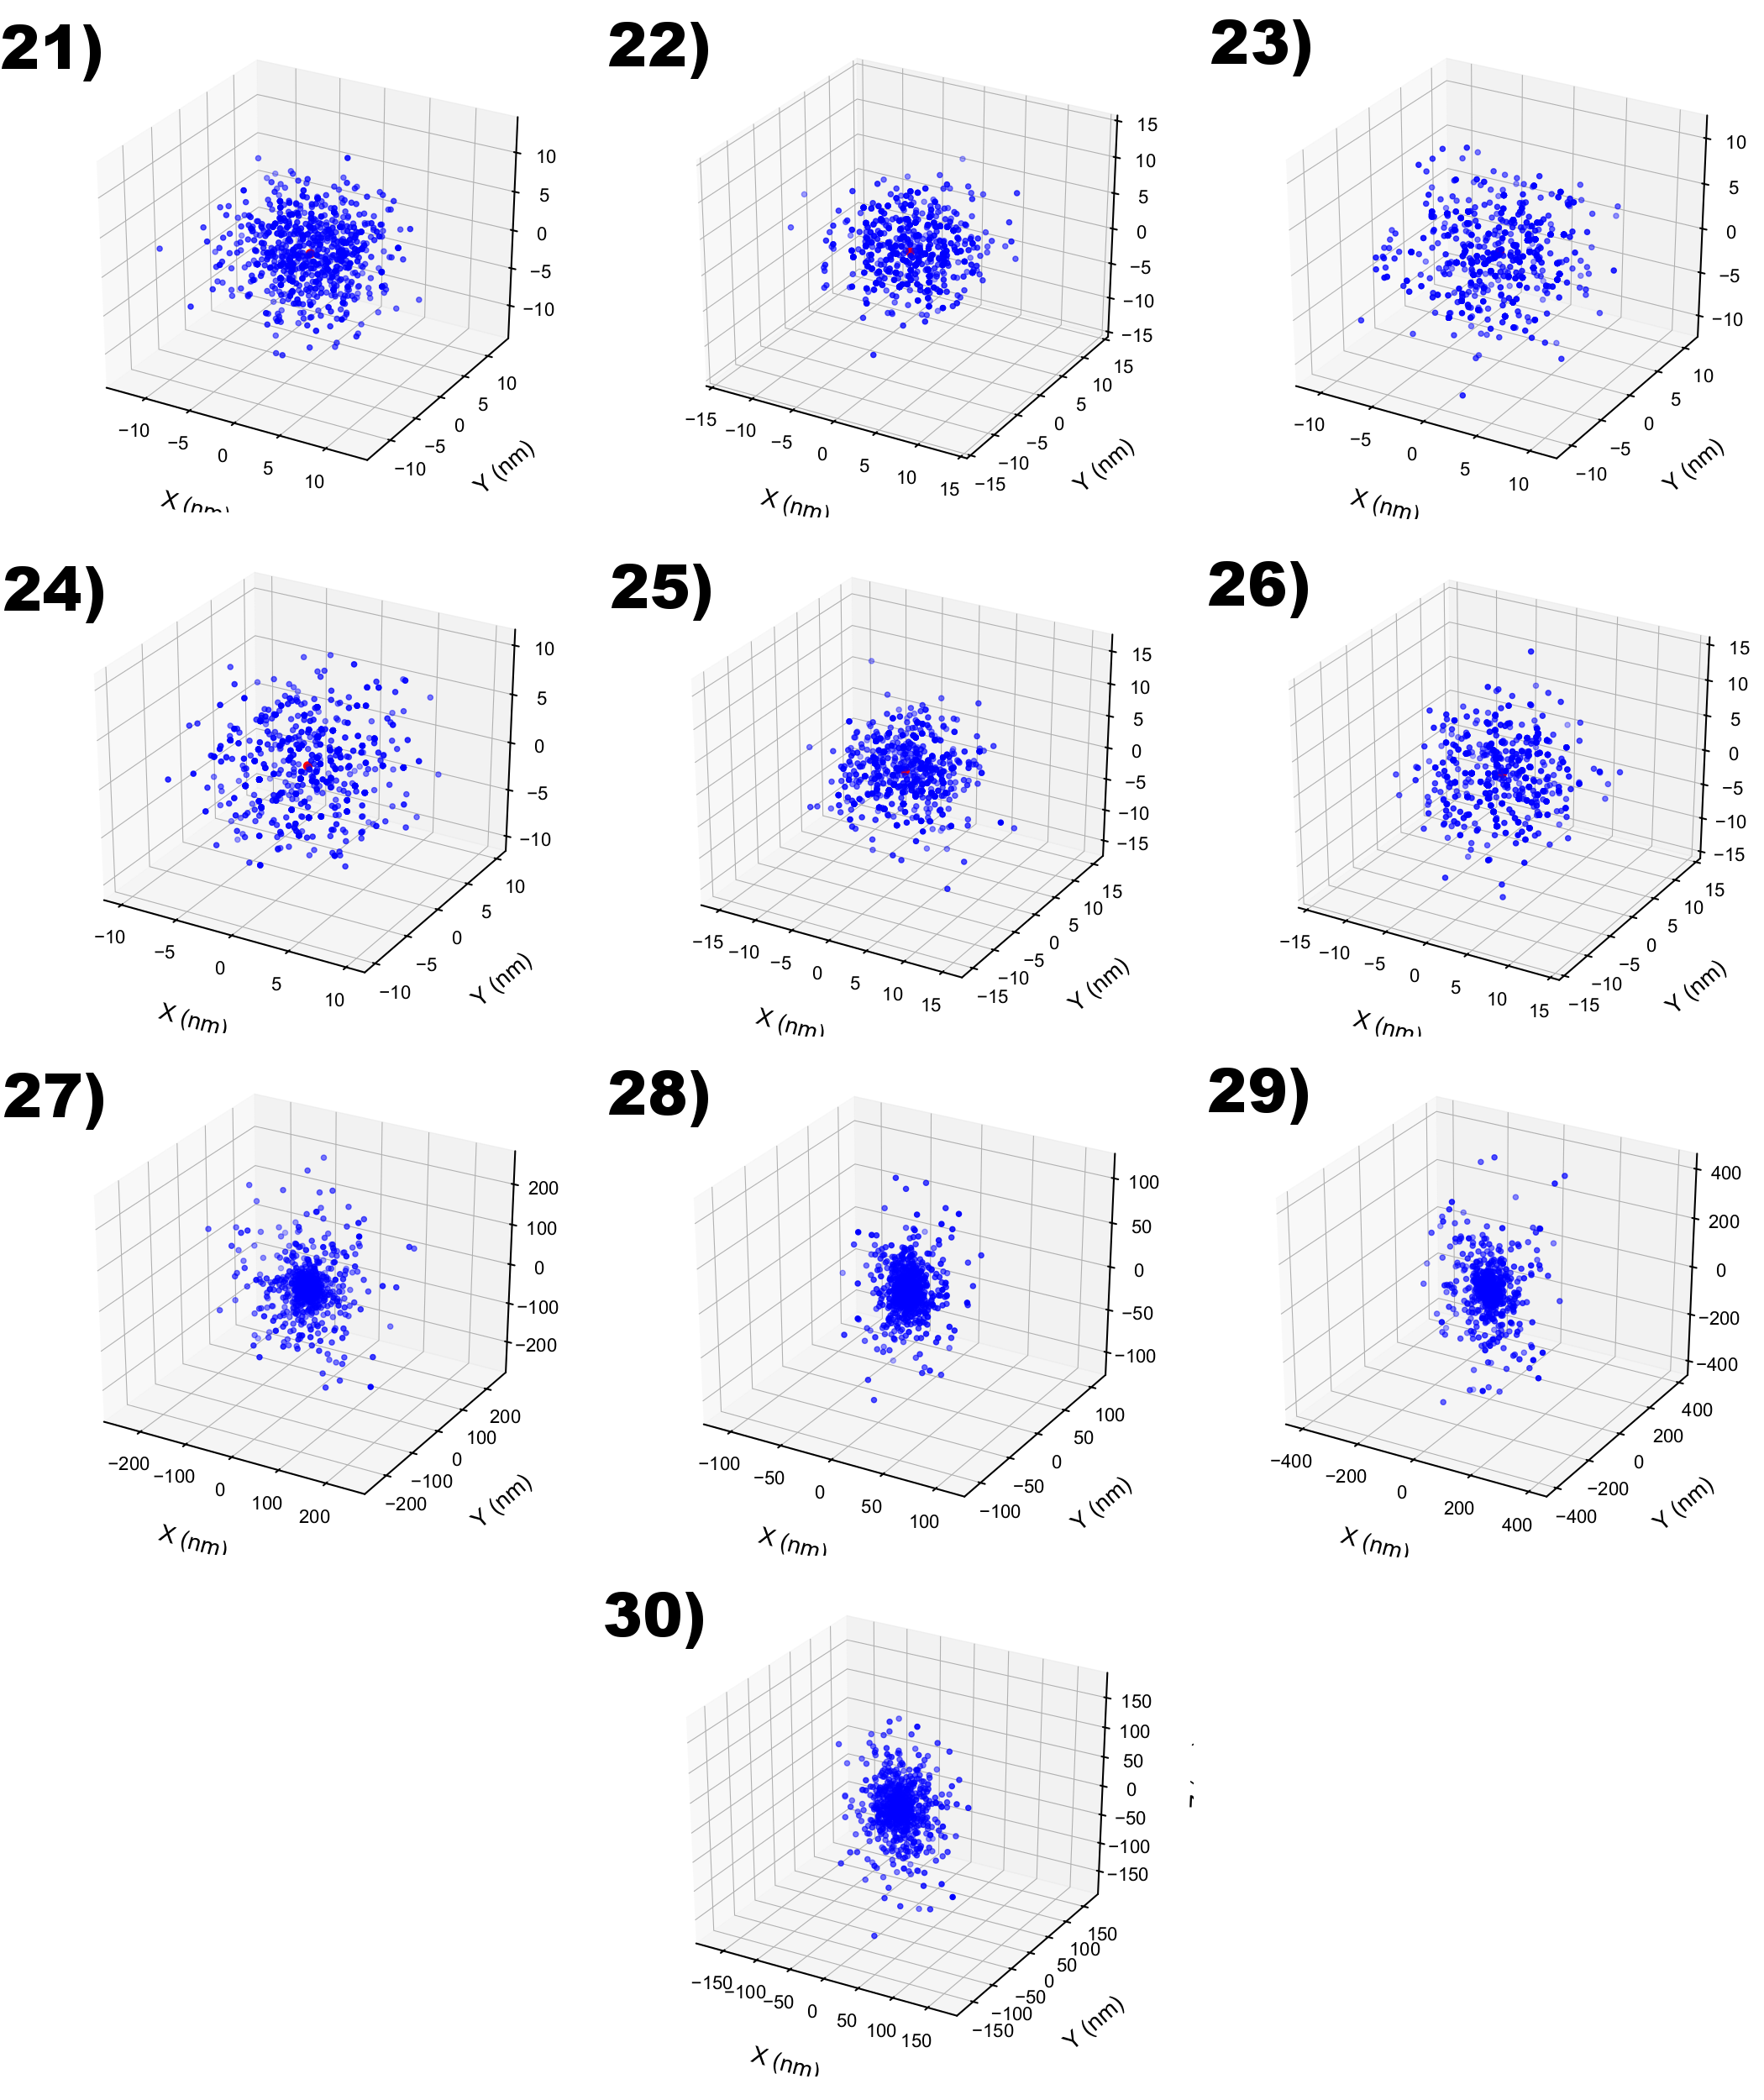
\includegraphics[width=\textwidth]{Figures/anisotropyHoleFrameOrig.png}
    \caption{The periodic anisotropies of the carrier transport within the morphologies \textbf{21} - \textbf{30}.}
	\label{fig:AnisFrameOrig}
\end{figure}

\clearpage
\subsection{MSDs}


\begin{figure}[h!]\centering
	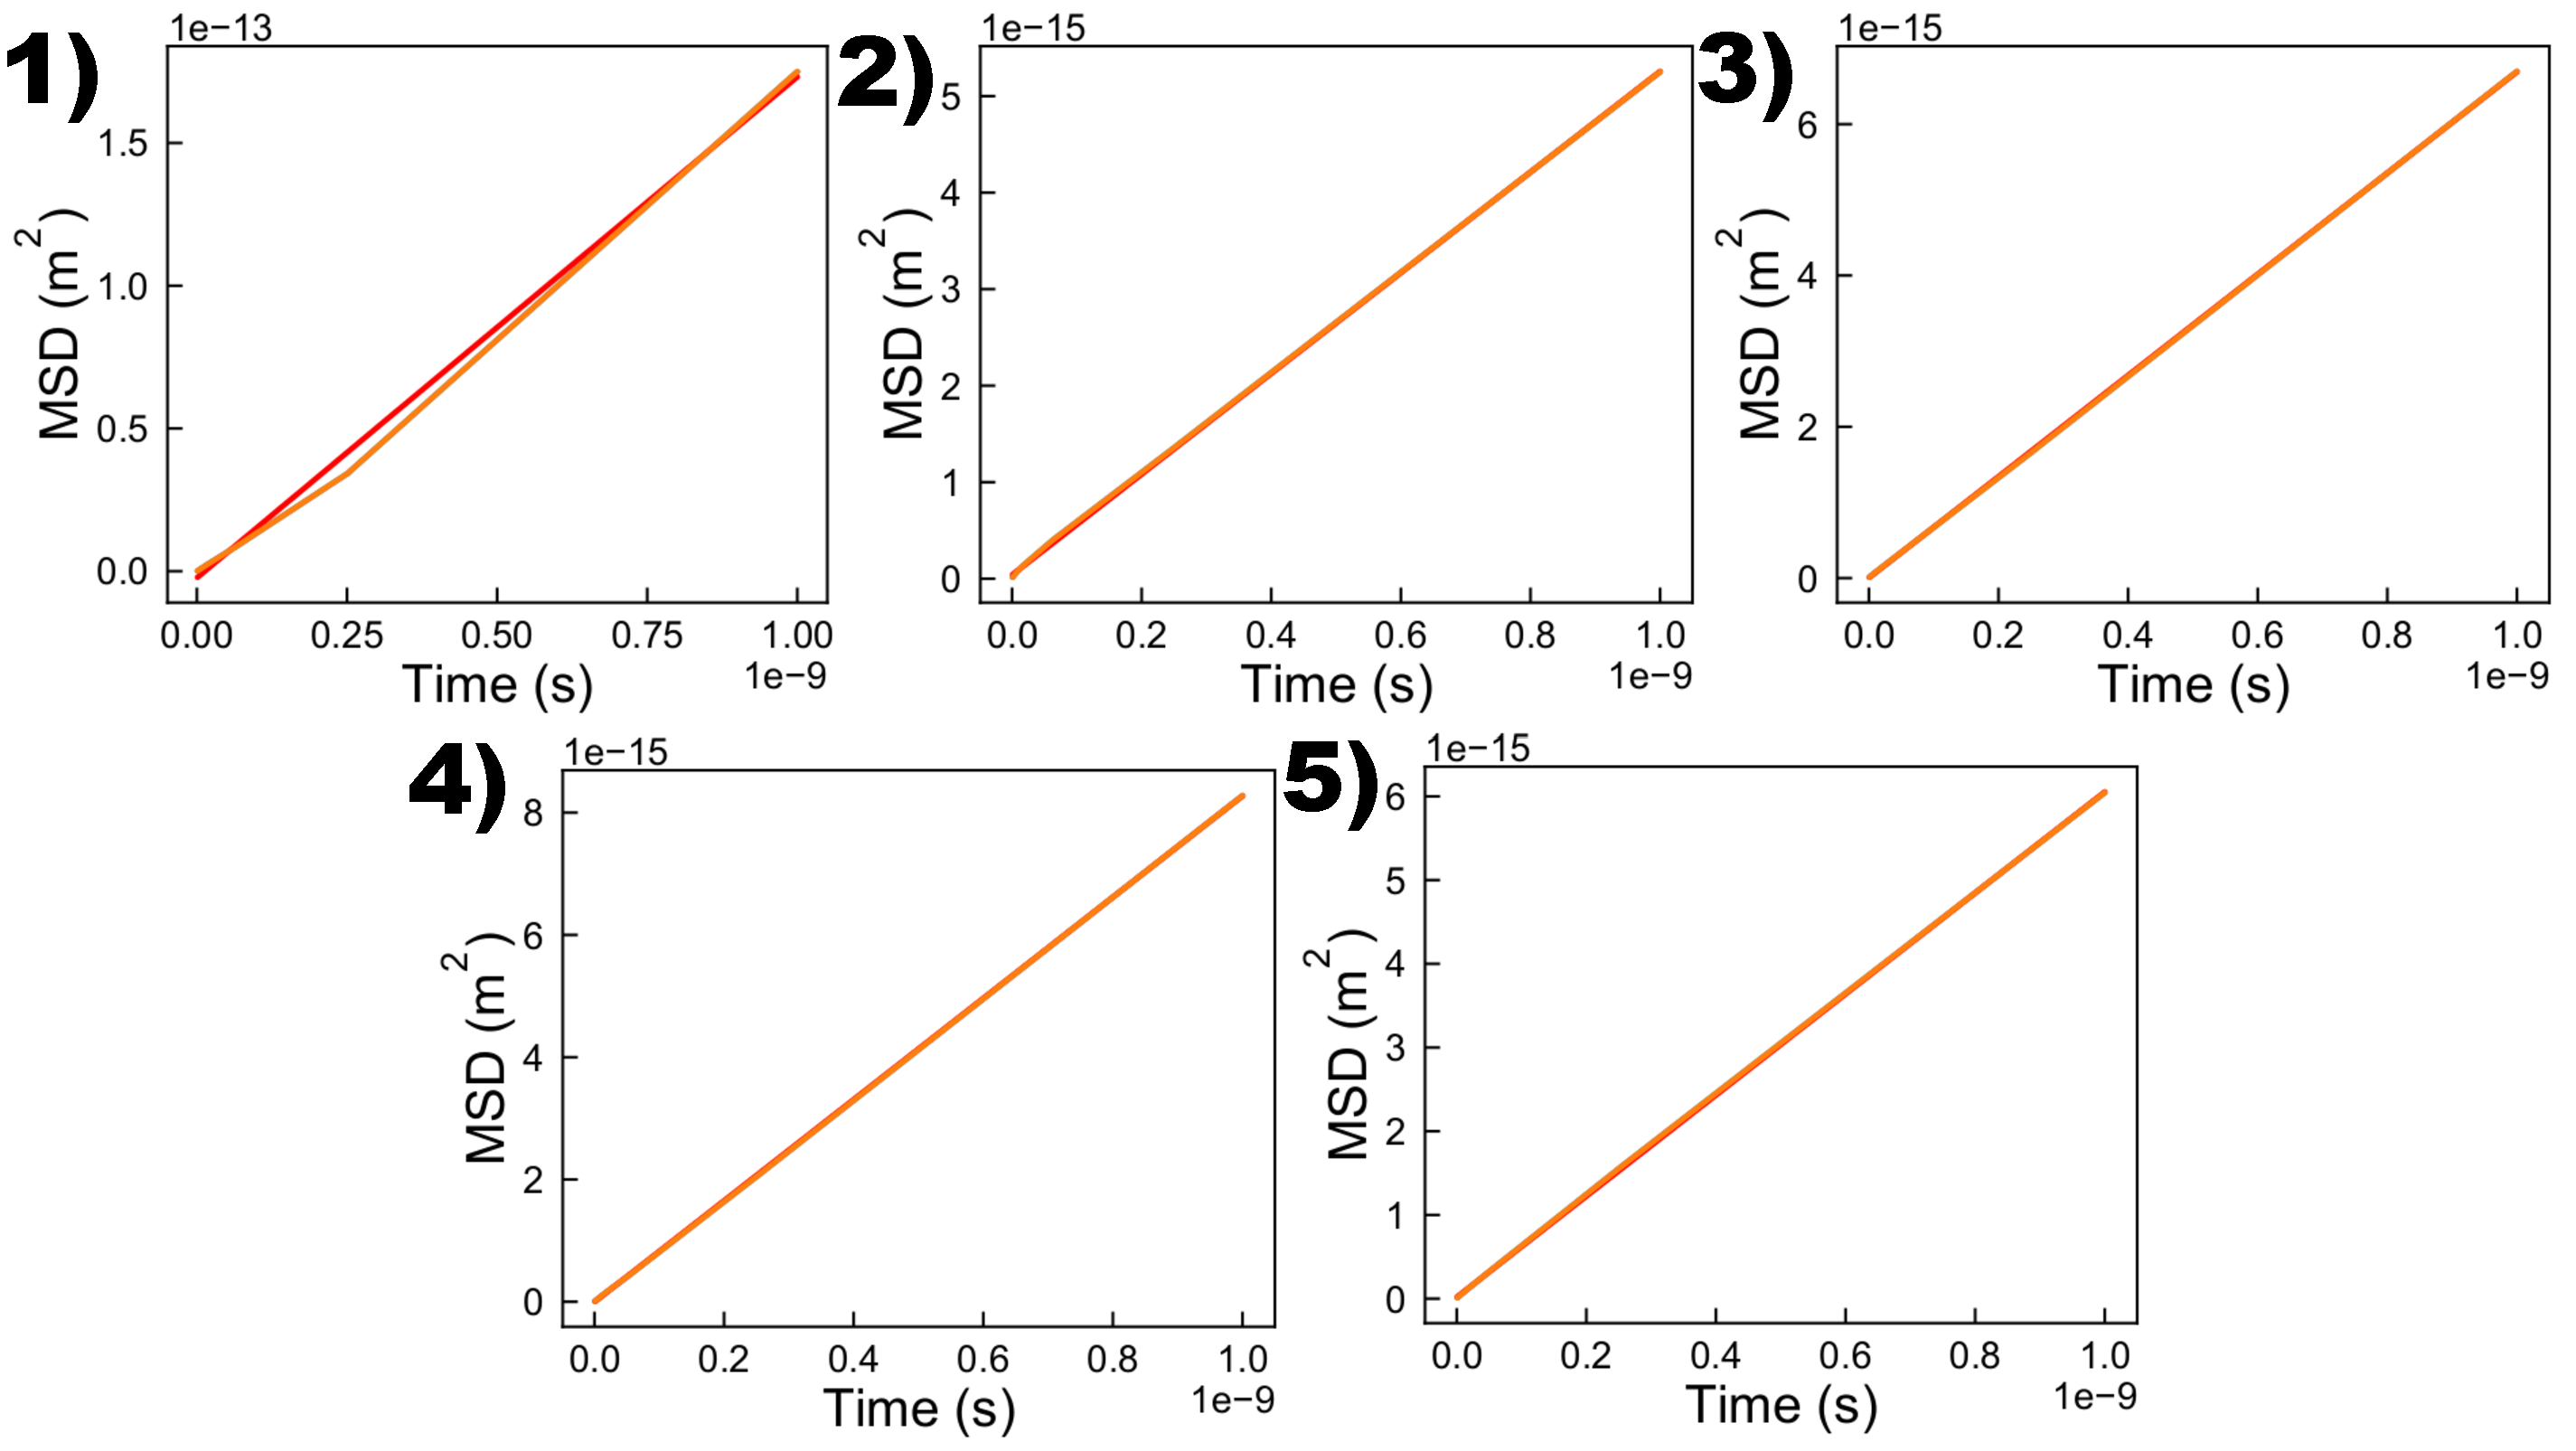
\includegraphics[width=\textwidth]{Figures/LinMSDHole.pdf}
    \caption{The linear mean squared displacement curves of the carriers within the morphologies \textbf{1} - \textbf{5}.}
	\label{fig:MSD}
\end{figure}


\begin{figure}[h!]\centering
	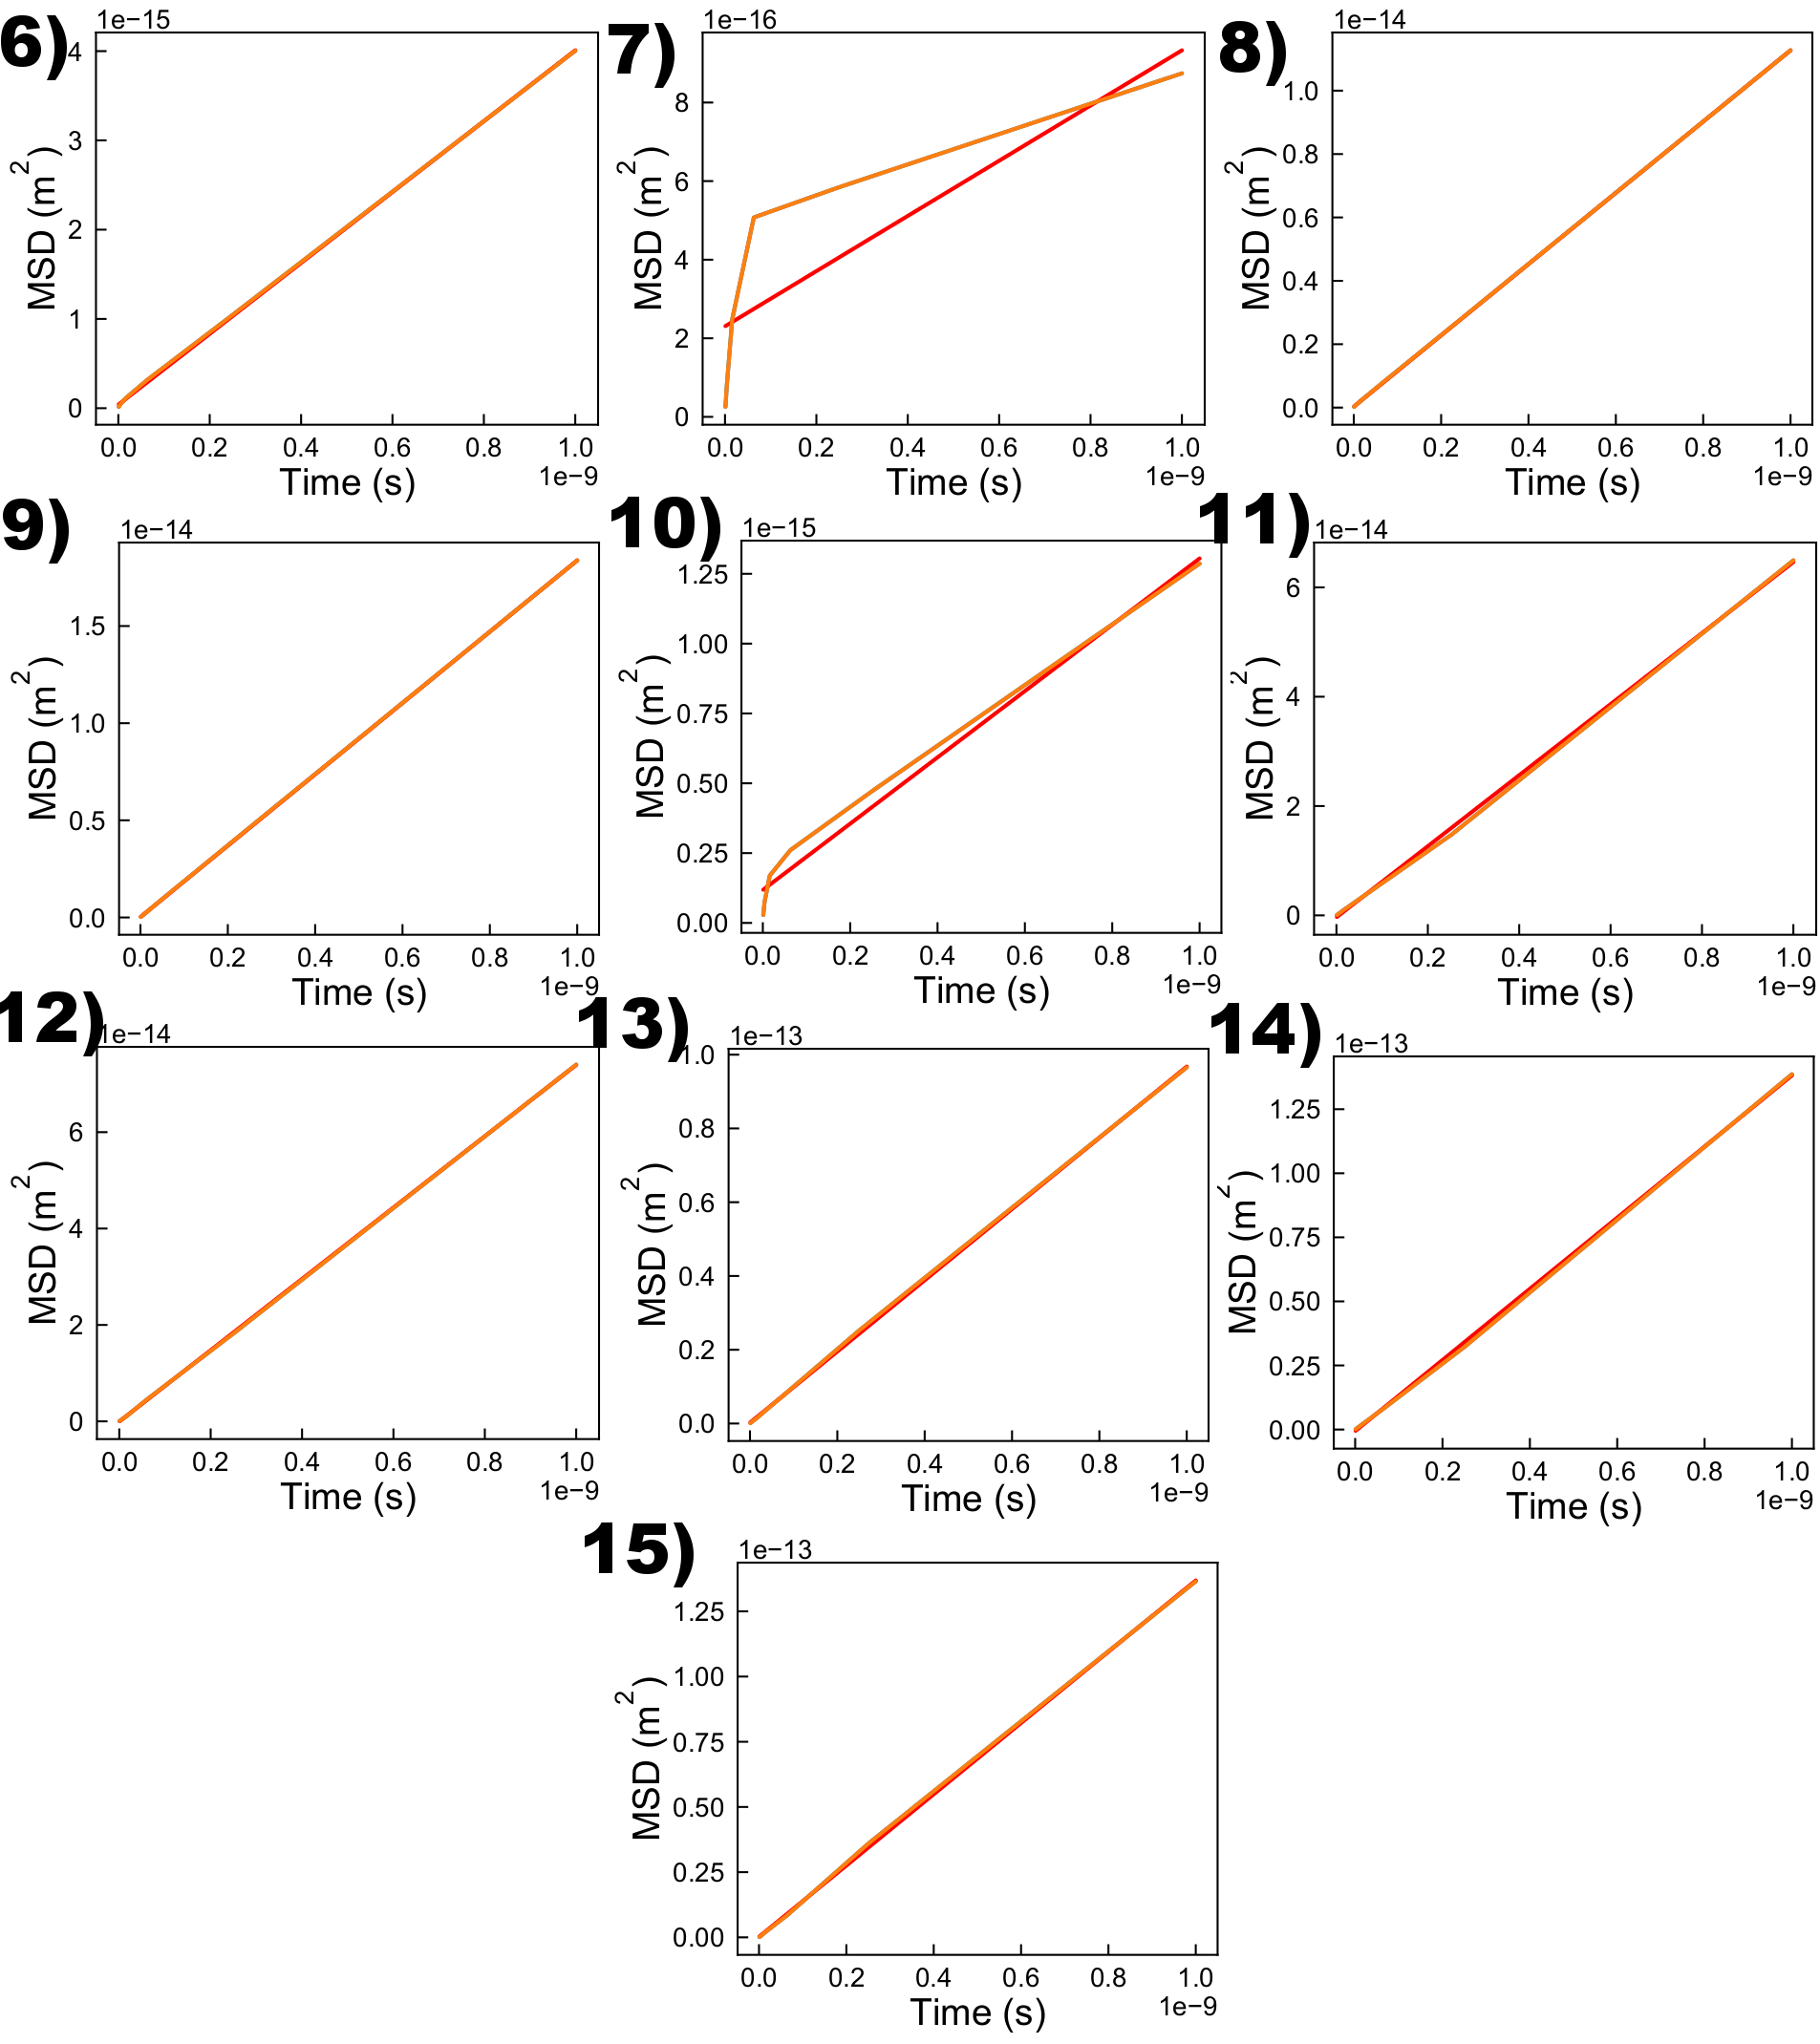
\includegraphics[width=\textwidth]{Figures/LinMSDHoleFrame.png}
    \caption{The linear mean squared displacement curves of the carriers within the morphologies \textbf{6} - \textbf{15}.}
	\label{fig:MSDFrame}
\end{figure}

\begin{figure}[h!]\centering
	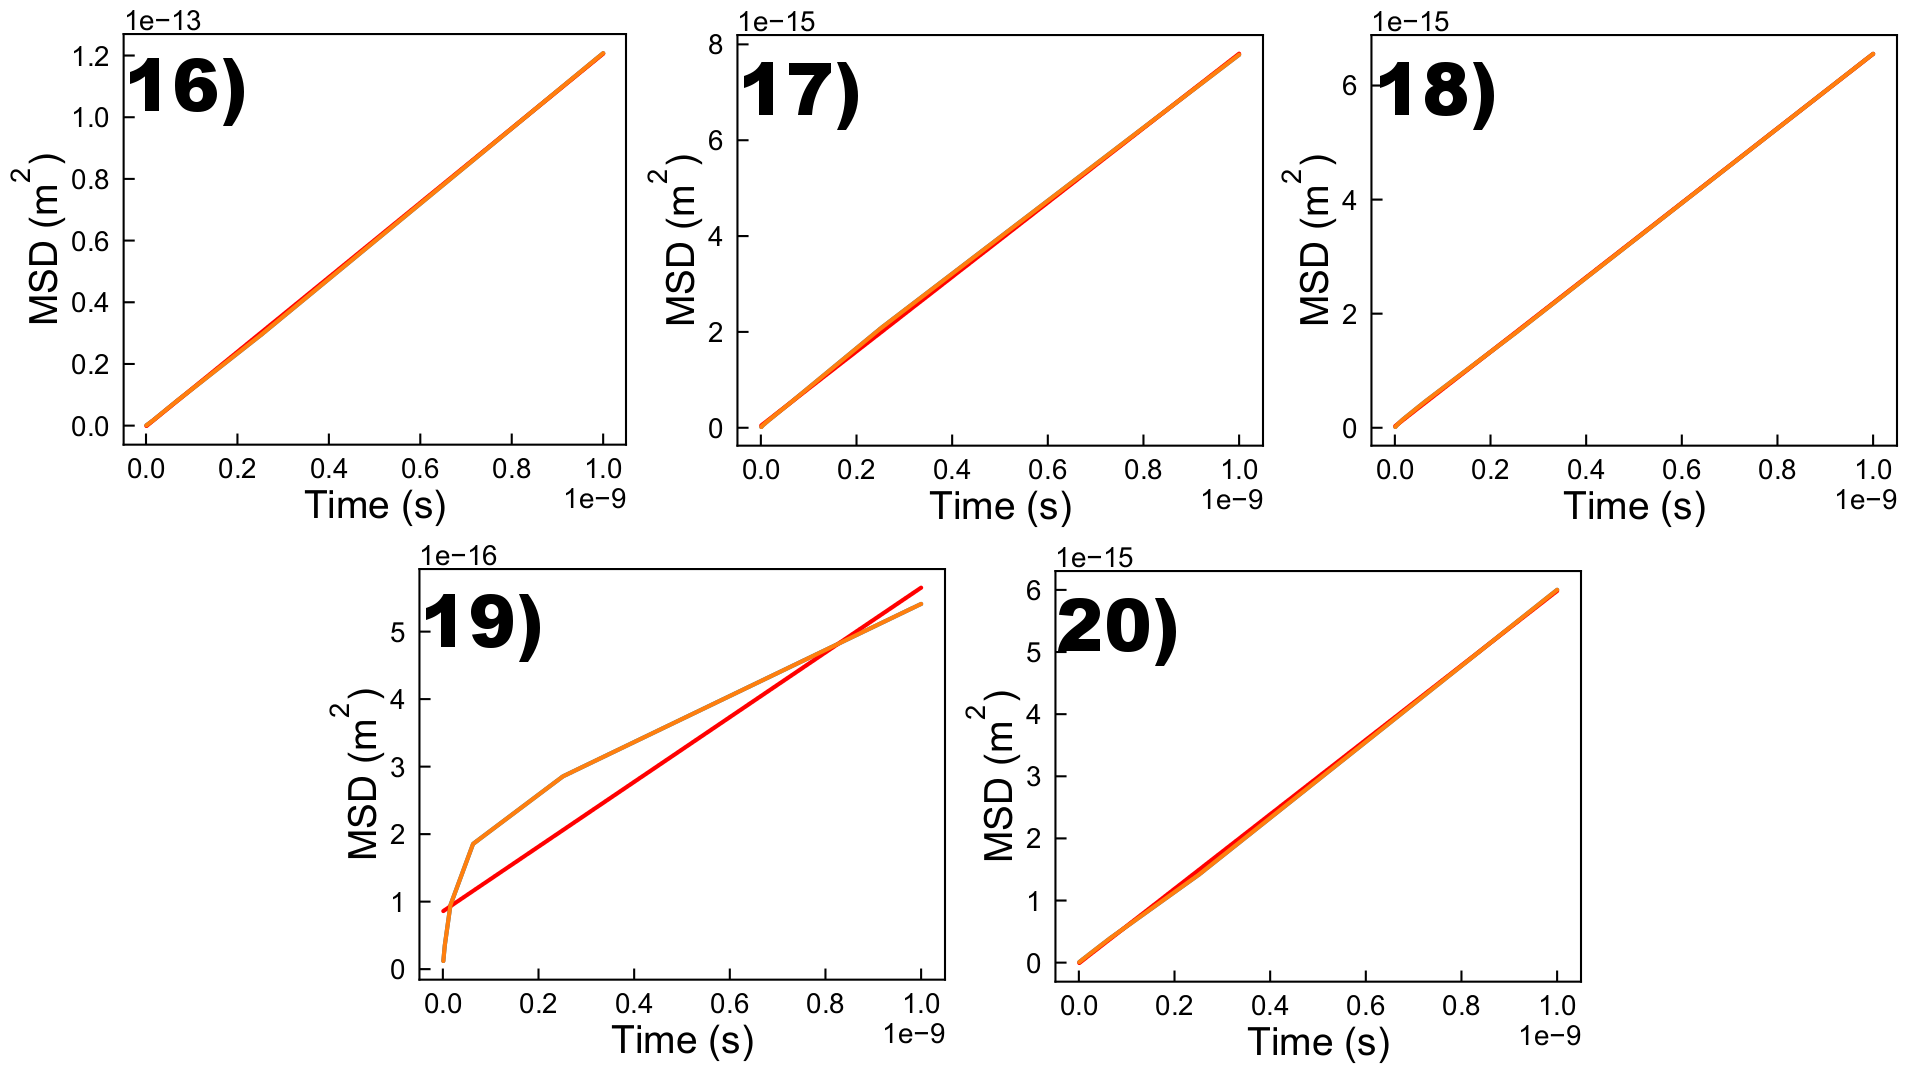
\includegraphics[width=\textwidth]{Figures/LinMSDHoleOrig.png}
    \caption{The linear mean squared displacement curves of the carriers within the morphologies \textbf{16} - \textbf{20}.}
	\label{fig:MSDOrig}
\end{figure}

\begin{figure}[h!]\centering
	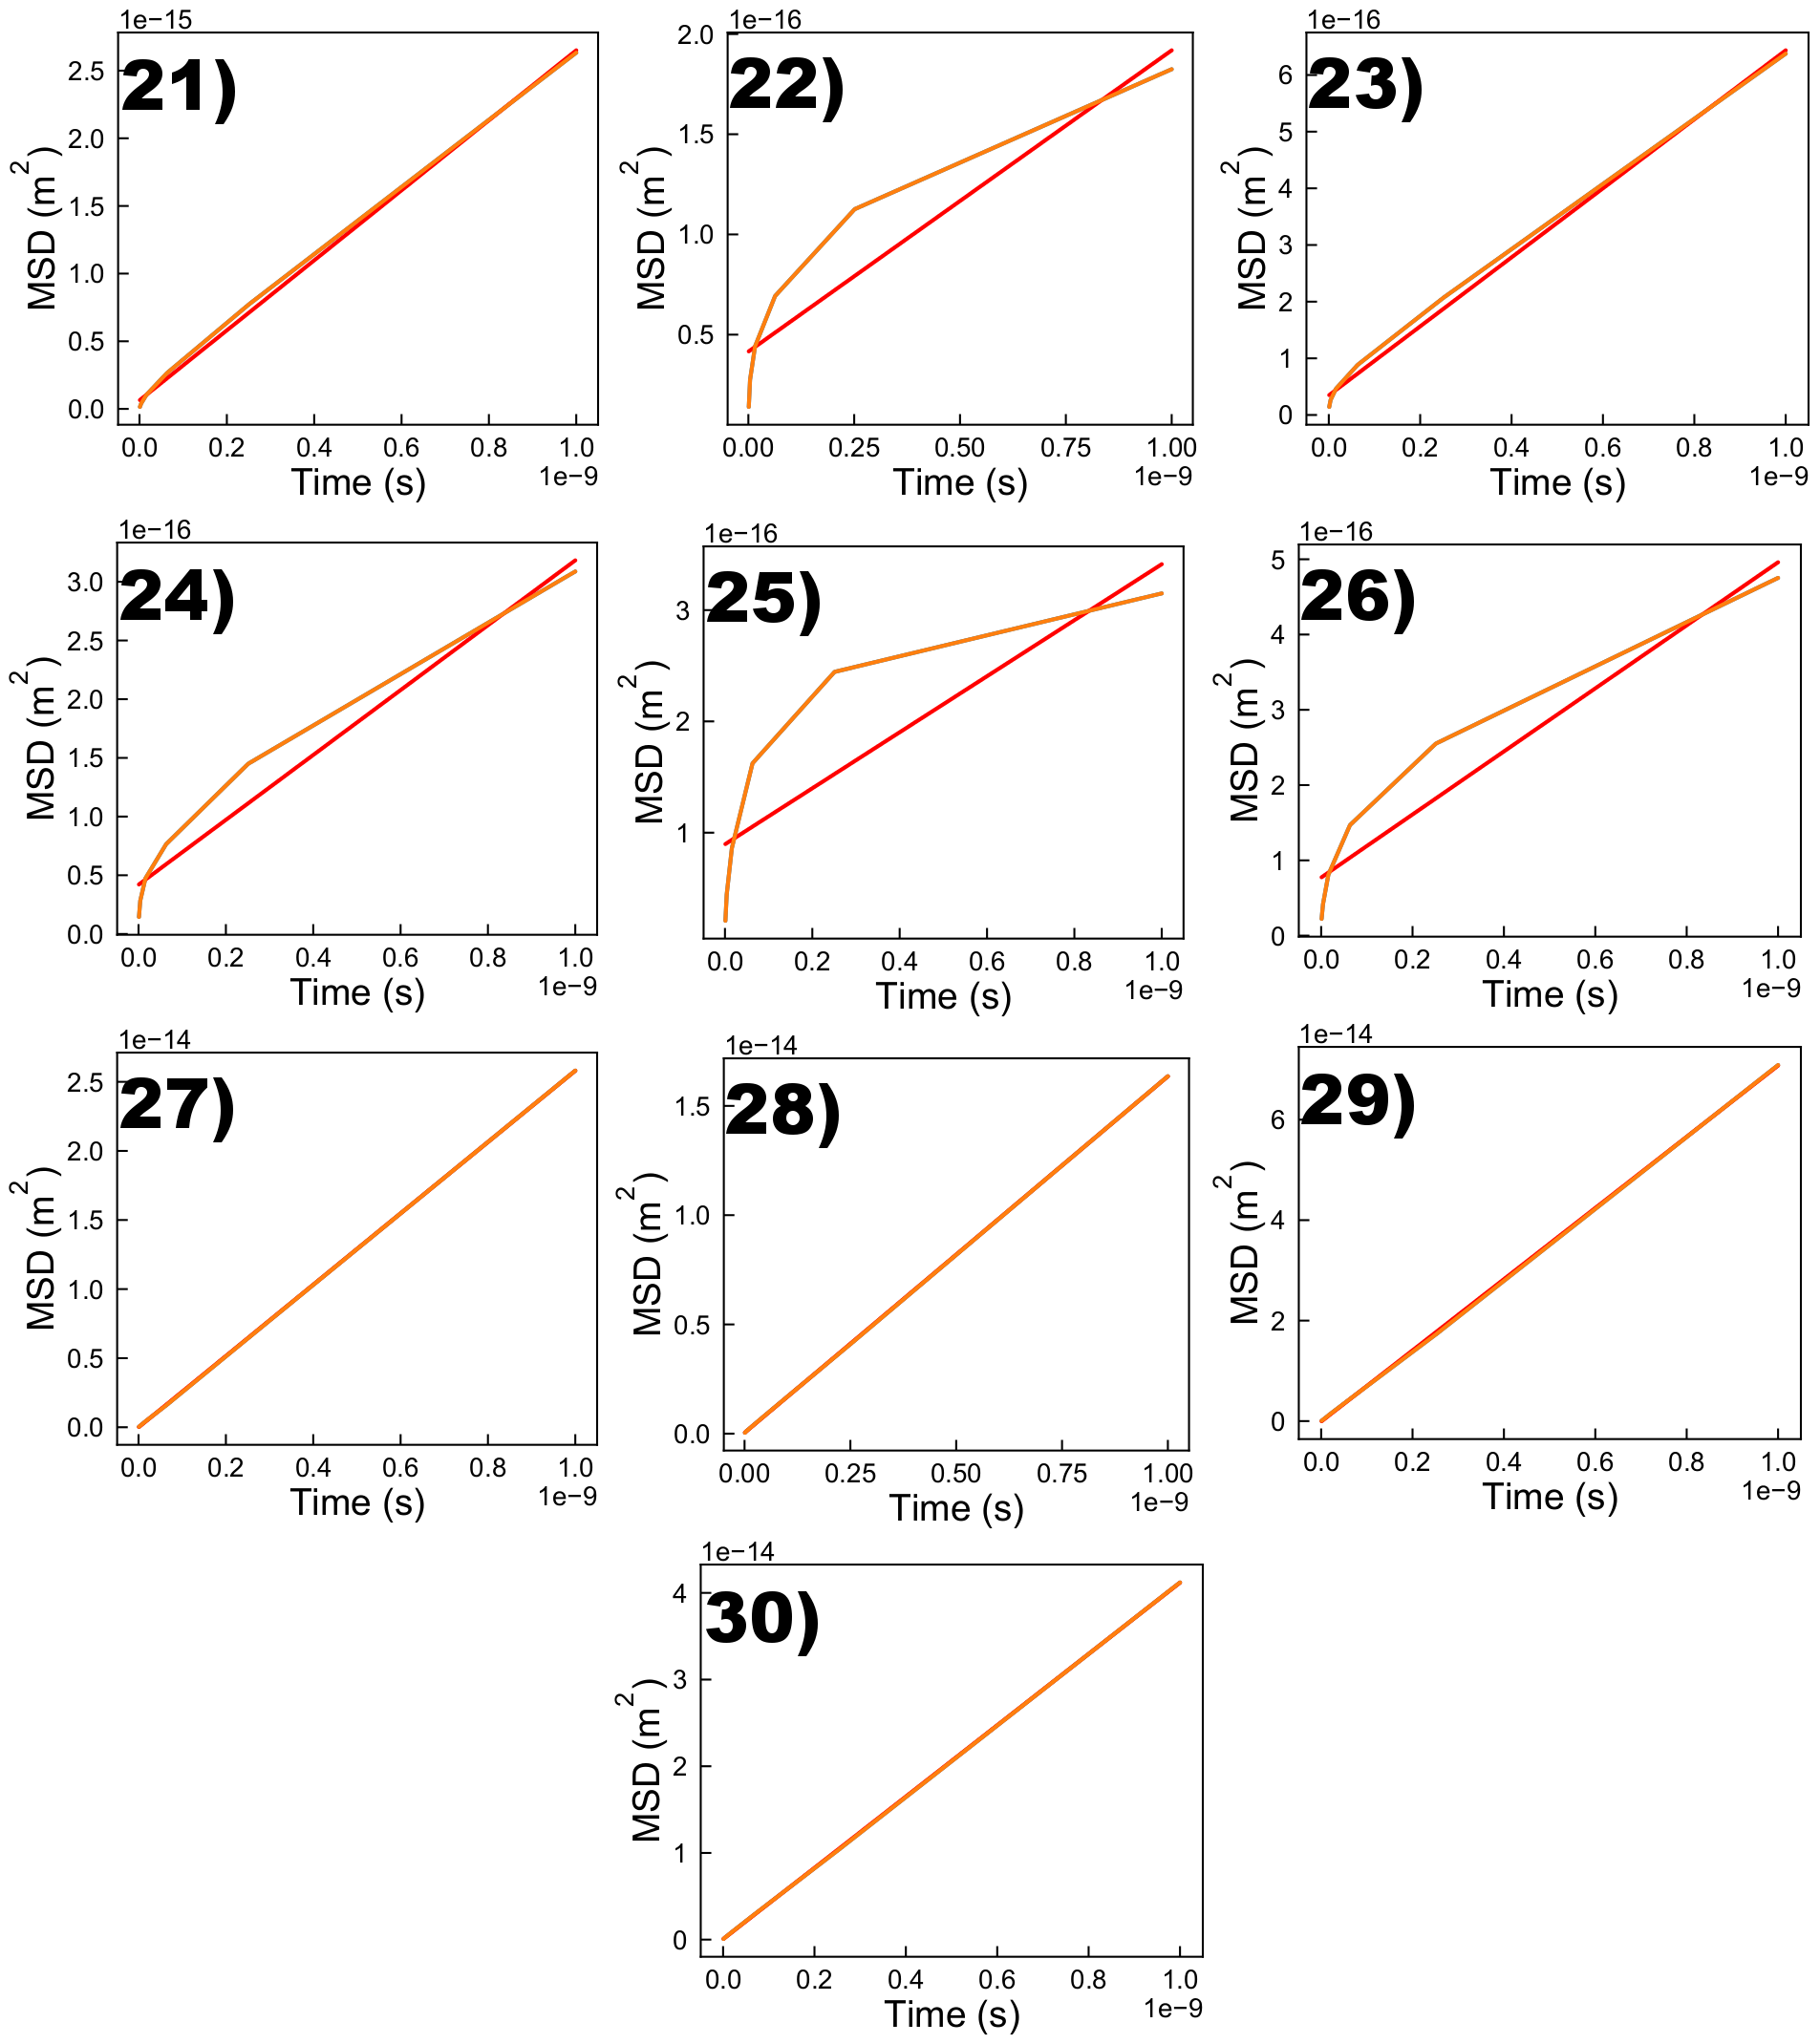
\includegraphics[width=\textwidth]{Figures/LinMSDHoleFrameOrig.png}
    \caption{The linear mean squared displacement curves of the carriers within the morphologies \textbf{21} - \textbf{30}.}
	\label{fig:MSDFrameOrig}
\end{figure}


\clearpage
\subsection{Hopping Rate Distributions}

\begin{figure}[h!]\centering
    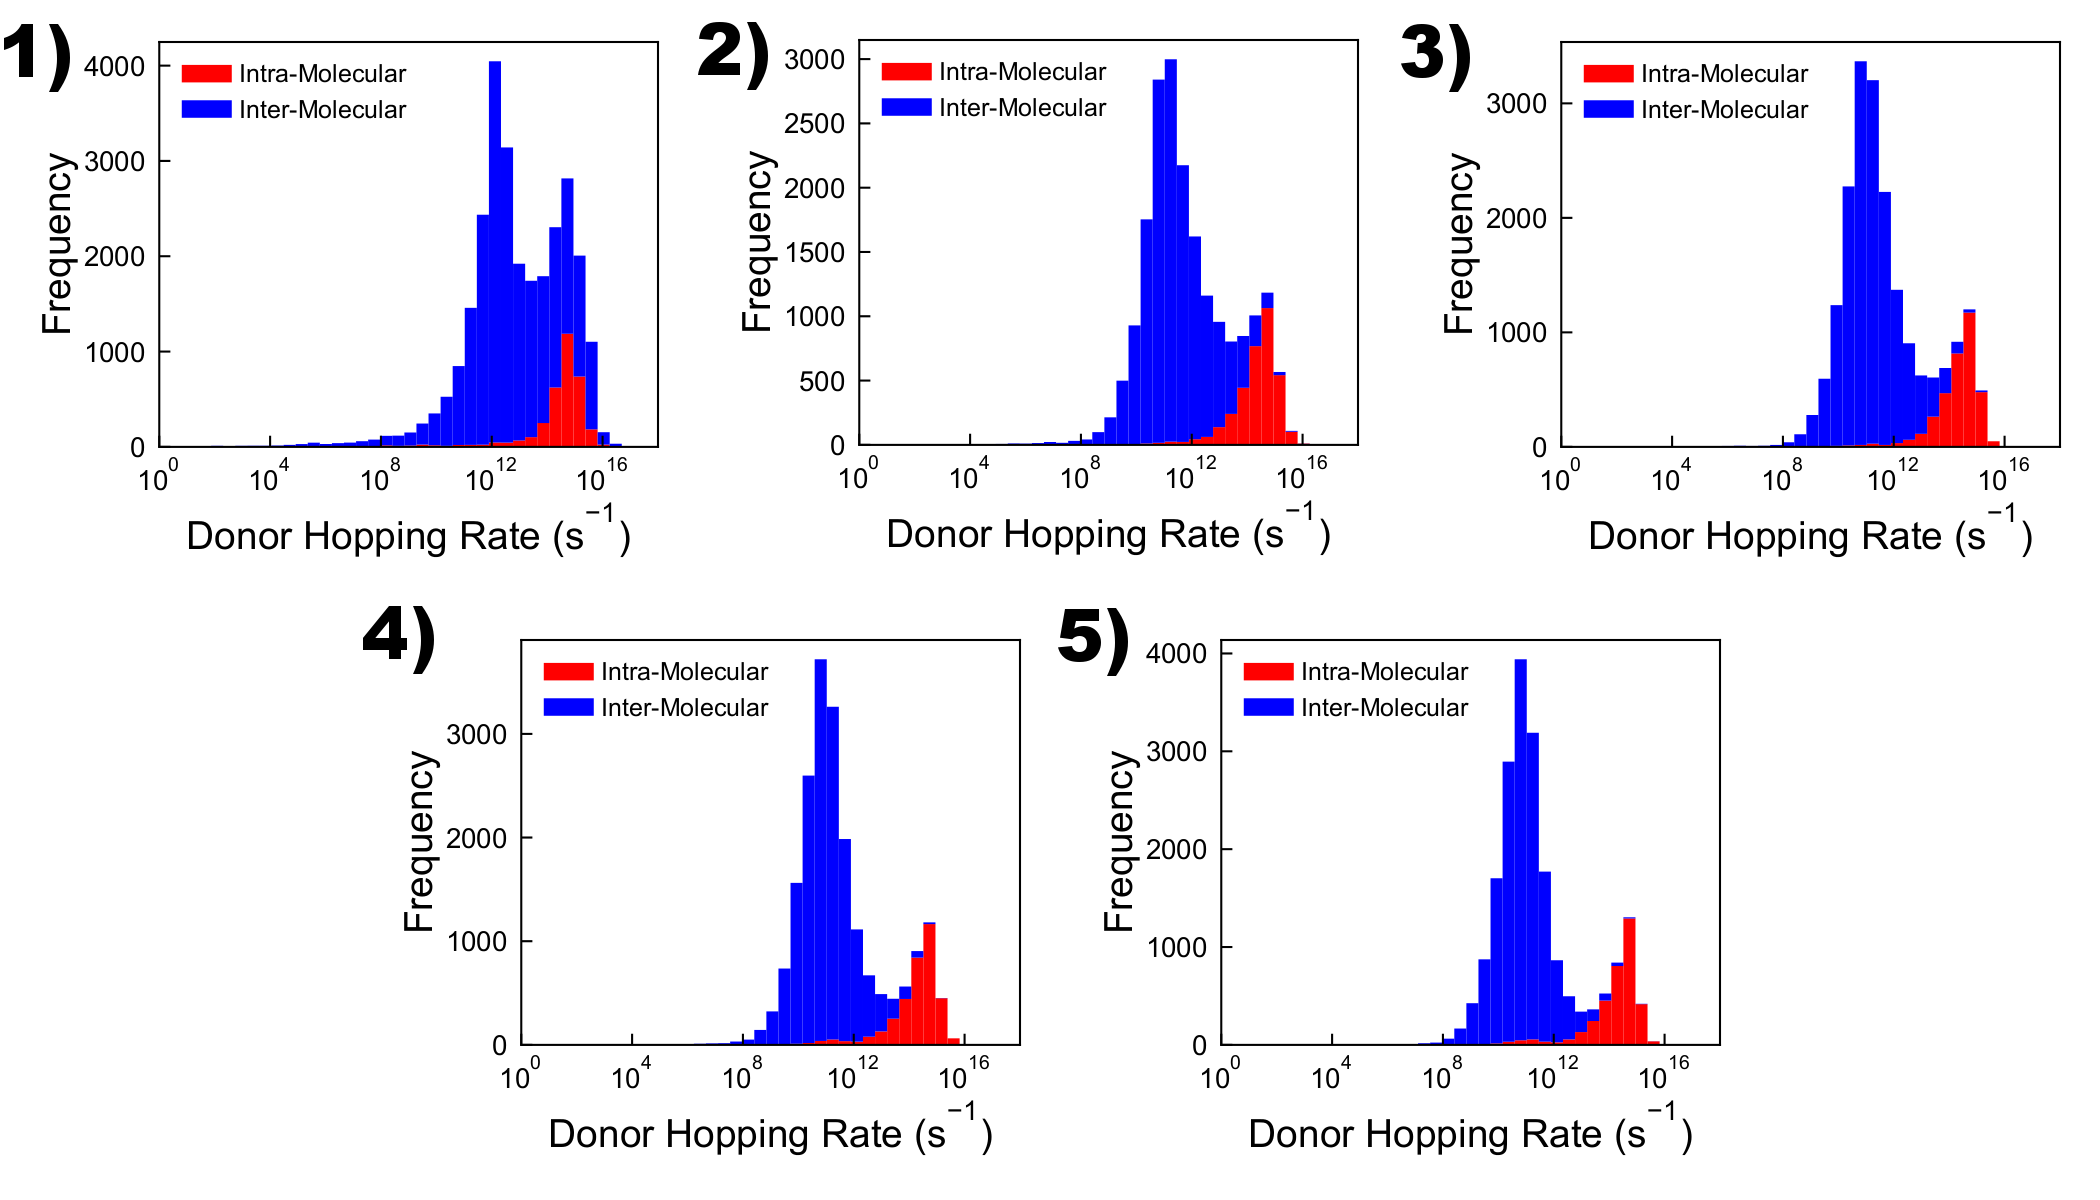
\includegraphics[width=\textwidth]{Figures/DonorHoppingRateMixed.png}
    \caption{The stacked hopping-rate distributions for intra- and inter-molecular hops executed by carriers within the morphologies \textbf{1} - \textbf{5}.}
	\label{fig:HoppingRateMixed}
\end{figure}

\begin{figure}[h!]\centering
    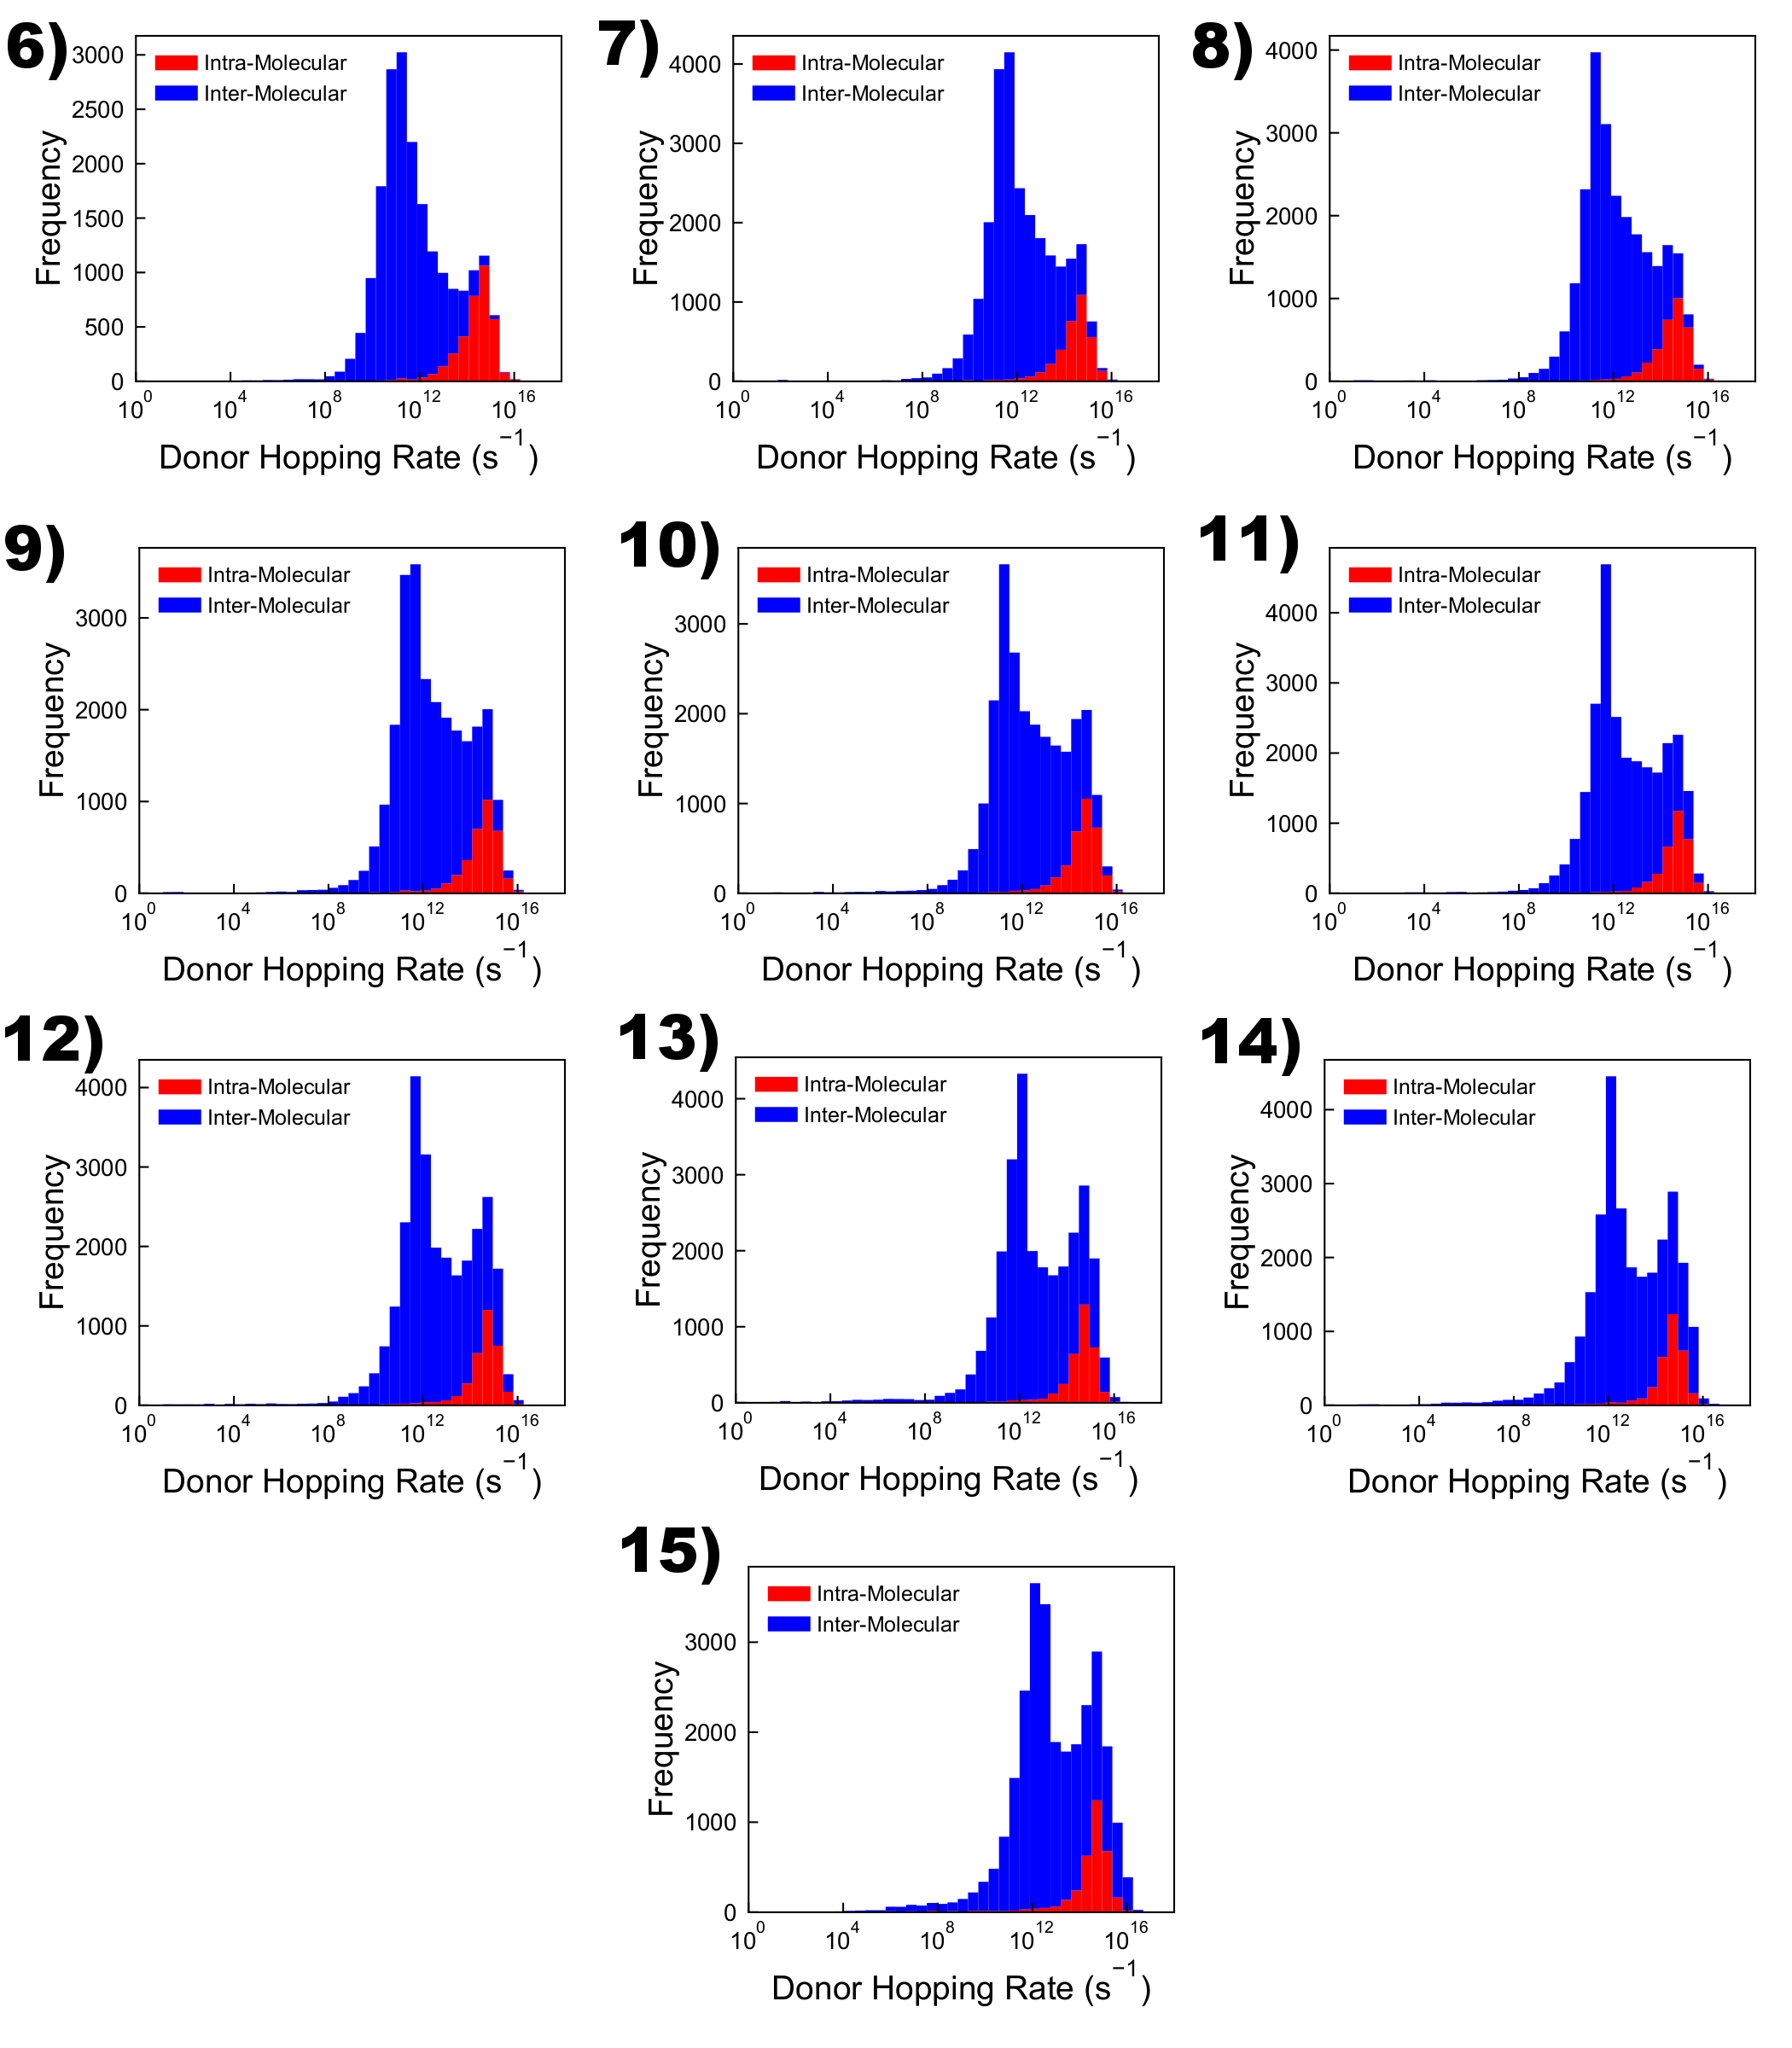
\includegraphics[width=\textwidth]{Figures/DonorHoppingRateMixedFrame.png}
    \caption{The stacked hopping-rate distributions for intra- and inter-molecular hops executed by carriers within the morphologies \textbf{6} - \textbf{15}.}
	\label{fig:HoppingRateMixedFrame}
\end{figure}

\begin{figure}[h!]\centering
    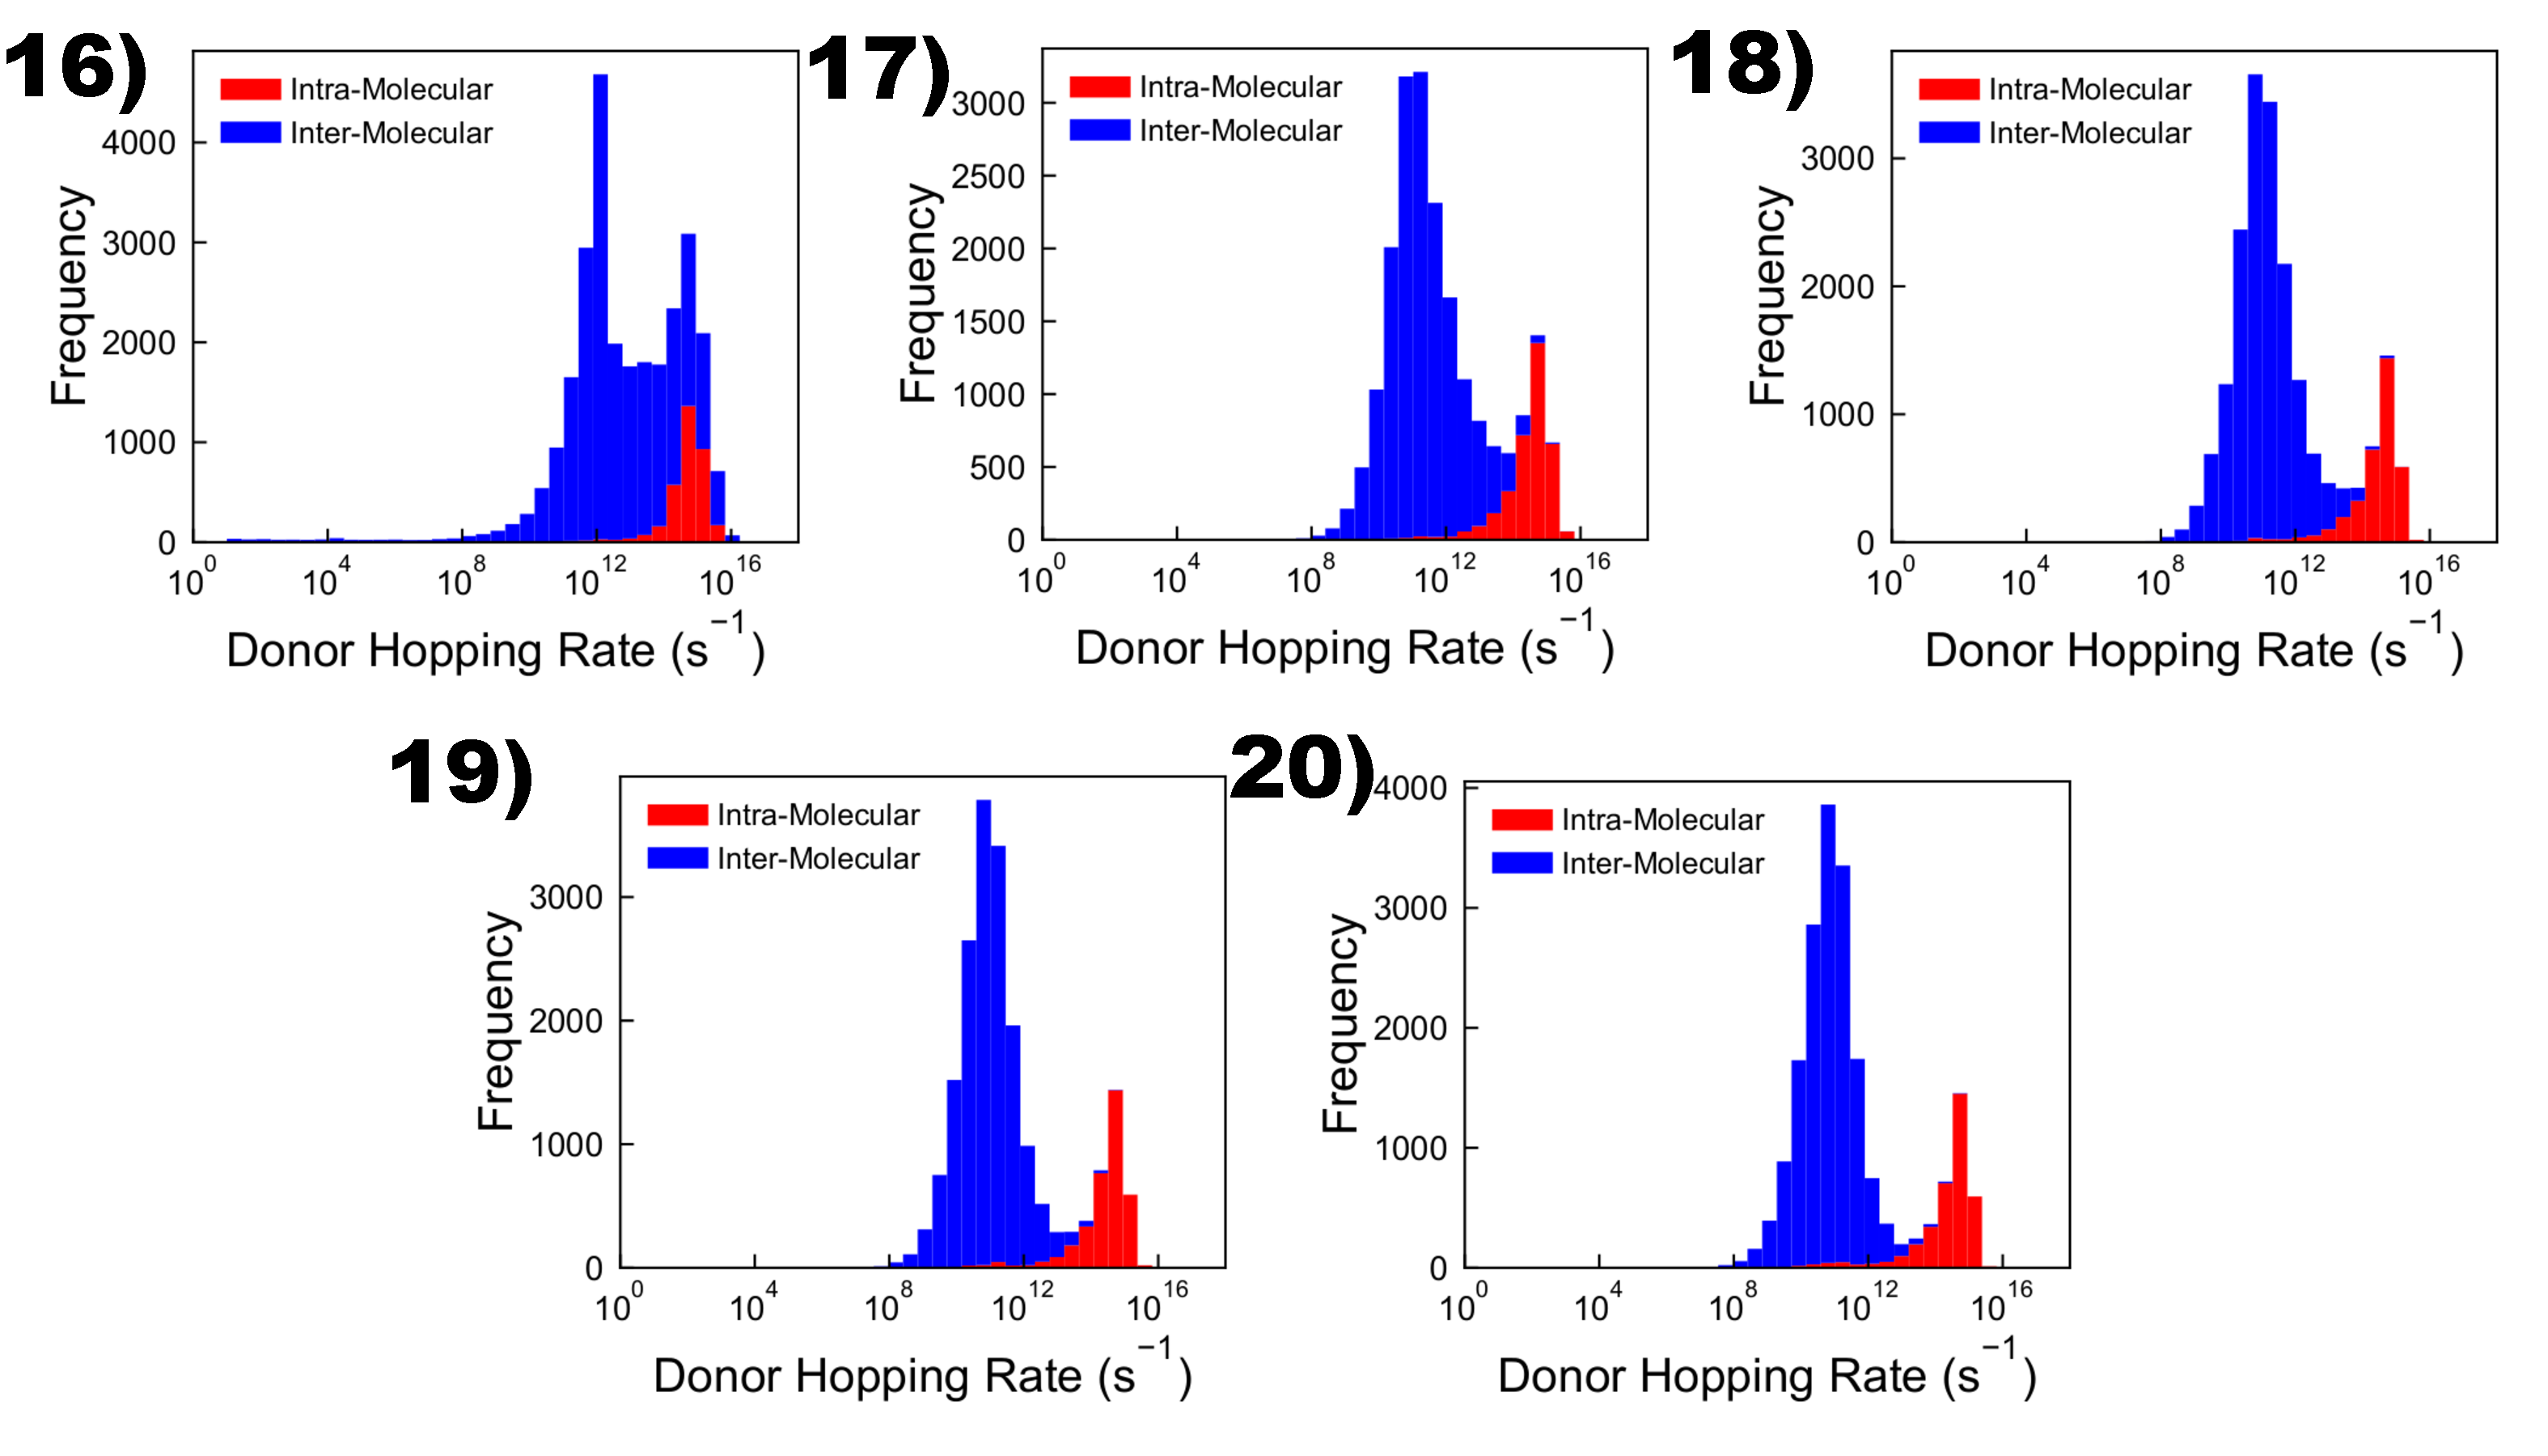
\includegraphics[width=\textwidth]{Figures/DonorHoppingRateMixedOrig.pdf}
    \caption{The stacked hopping-rate distributions for intra- and inter-molecular hops executed by carriers within the morphologies \textbf{16} - \textbf{20}.}
	\label{fig:HoppingRateMixedOrig}
\end{figure}

\begin{figure}[h!]\centering
    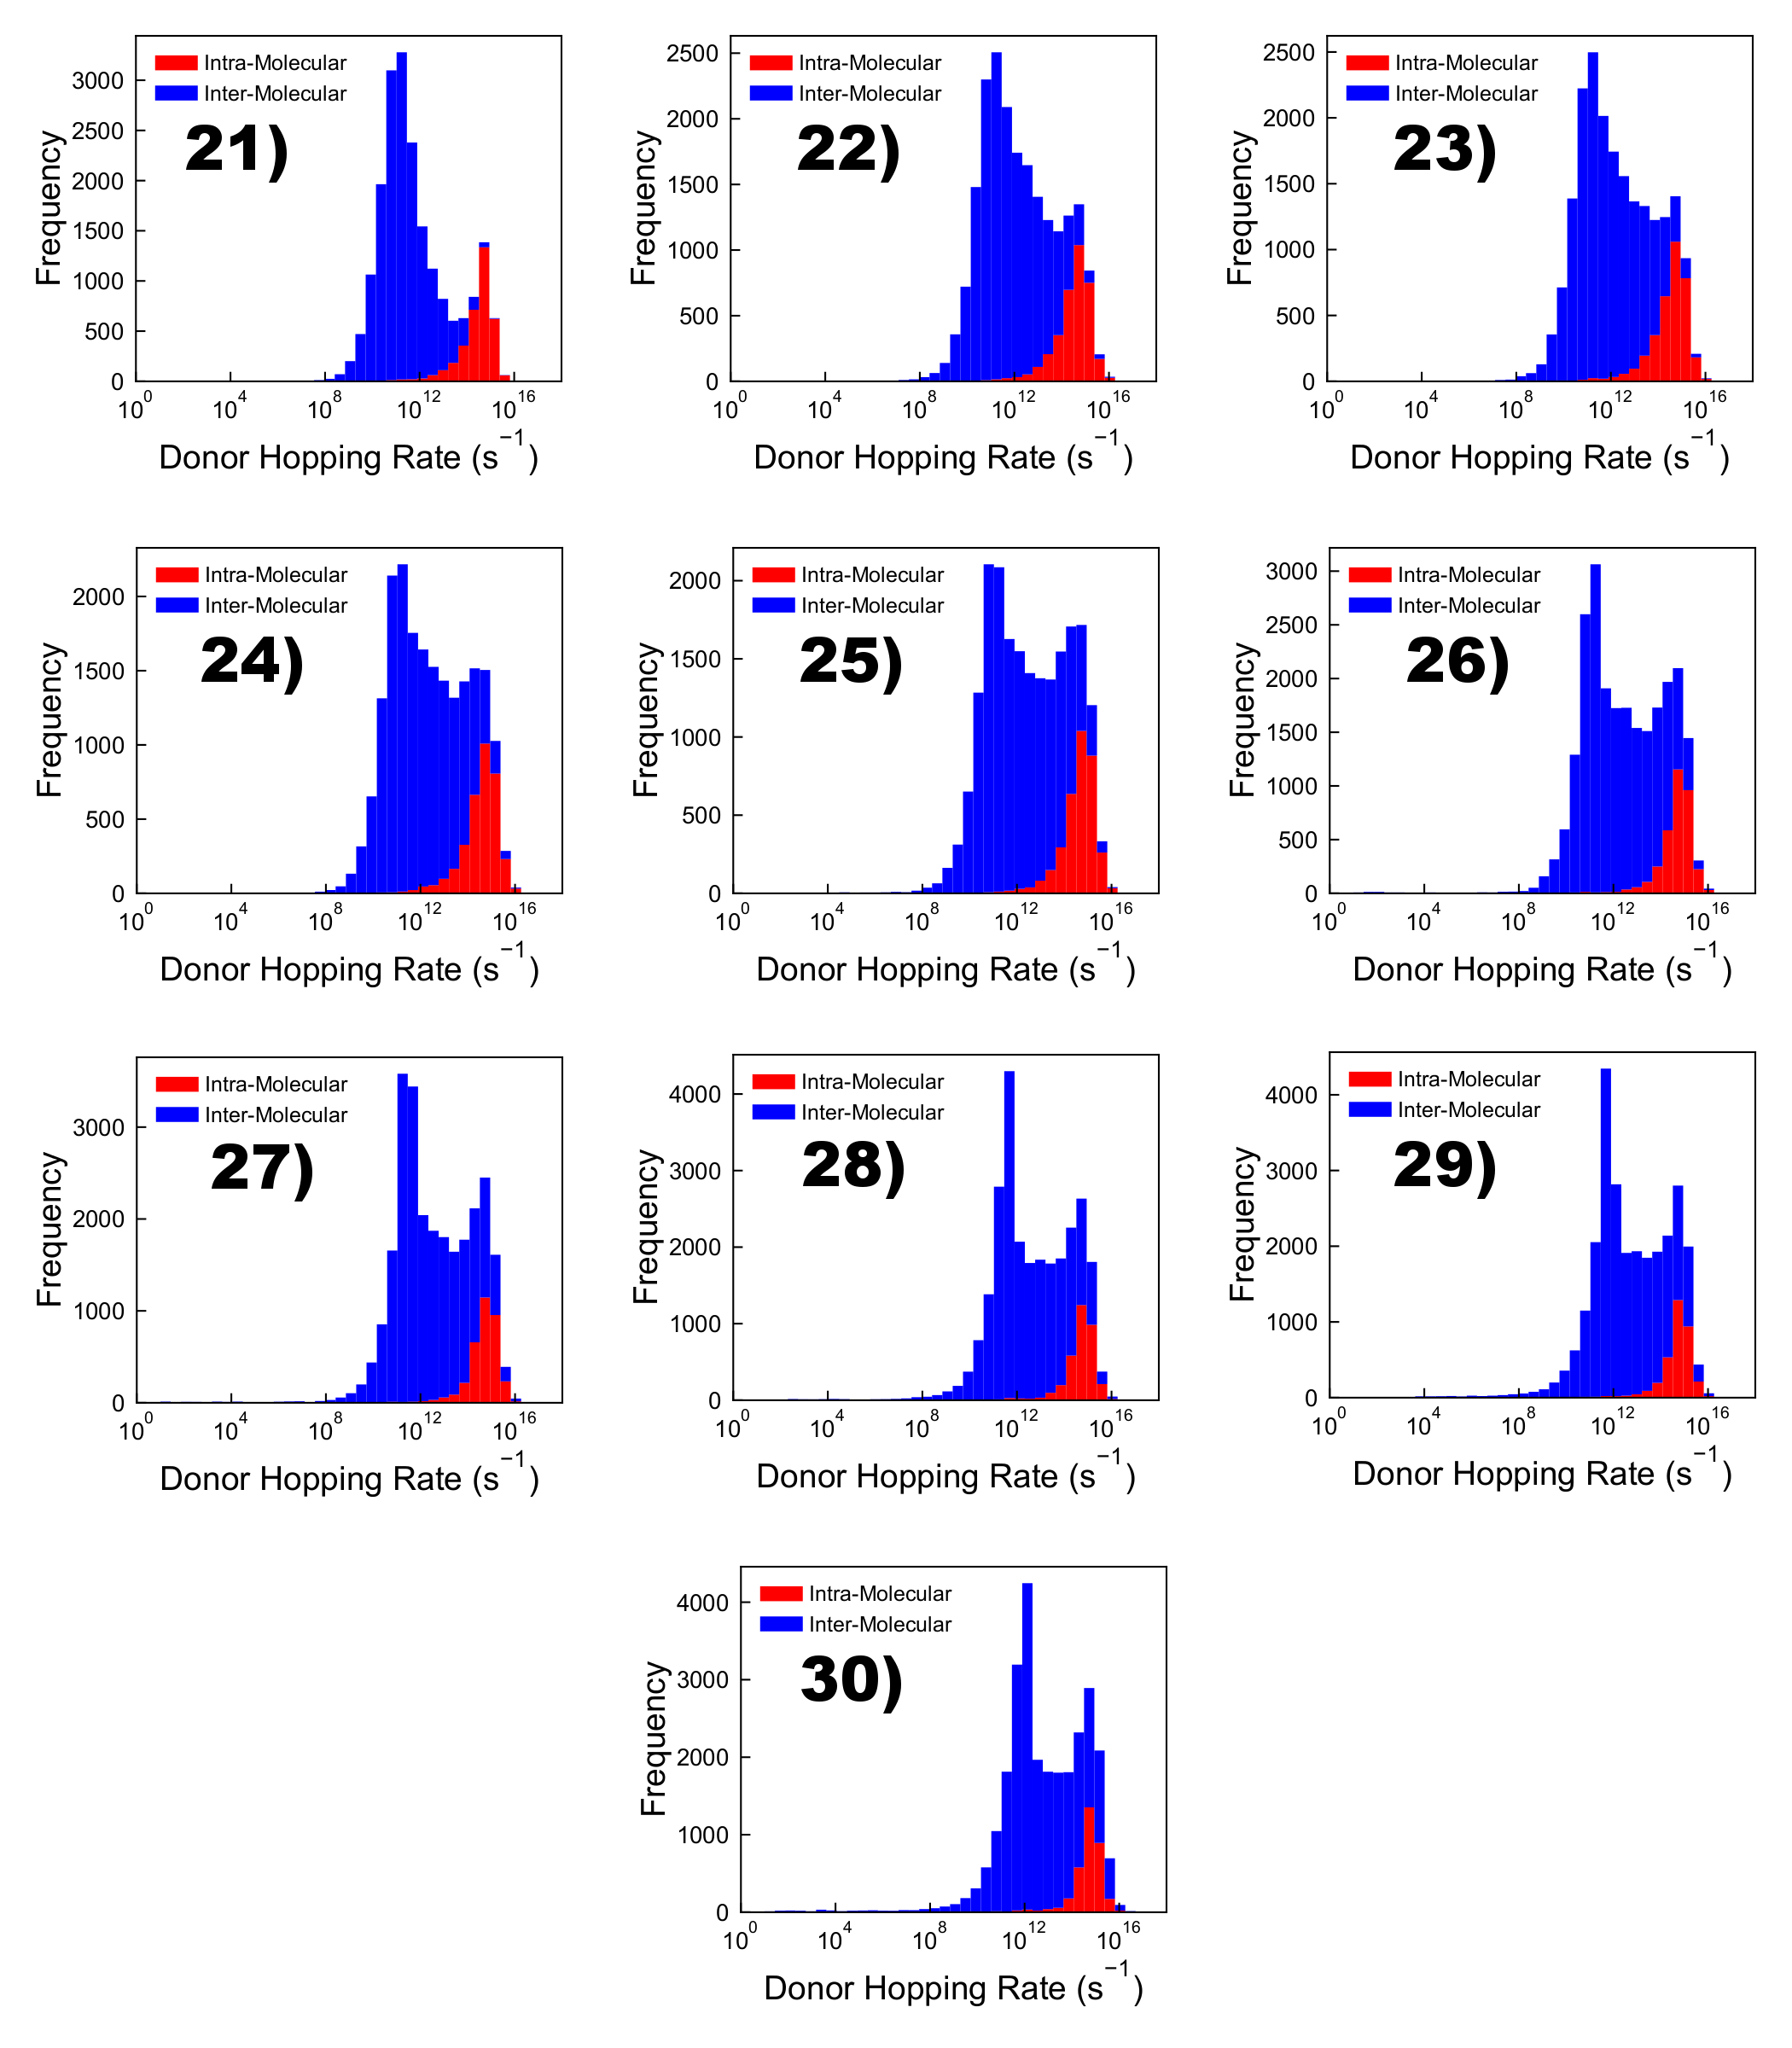
\includegraphics[width=\textwidth]{Figures/DonorHoppingRateMixedFrameOrig.png}
    \caption{The stacked hopping-rate distributions for intra- and inter-molecular hops executed by carriers within the morphologies \textbf{21} - \textbf{30}.}
	\label{fig:HoppingRateMixedFrameOrig}
\end{figure}

\clearpage


\bibliography{refs}
\bibliographystyle{unsrt}


\end{document}
